% Intended LaTeX compiler: xelatex
% All slides live in this file. Move a complete BEGIN FRAME / END FRAME block to reorder.
% Images stay in assets/. slides.org is historical notes, not the live source.
\documentclass[aspectratio=169,10pt]{beamer}
\usepackage{graphicx}
\usepackage{longtable}
\usepackage{wrapfig}
\usepackage{rotating}
\usepackage[normalem]{ulem}
\usepackage{amsmath}
\usepackage{amssymb}
\usepackage{hyperref}
\usepackage{fontspec}
\usepackage{array}
\setsansfont{FiraSans-Regular.otf}[BoldFont=FiraSans-Bold.otf,ItalicFont=FiraSans-Italic.otf,BoldItalicFont=FiraSans-BoldItalic.otf]
\AtBeginDocument{\AtBeginSection[]{}}
\institute{Carpenter-Shen Lab, Purdue University}
\usetheme{moloch}
\author{Alán F. Muñoz}
\date{10 November 2026}
\title{Uncovering biological relationships through morphological profiling: The JUMP-Cell Painting dataset and tools}
\subtitle{}
\hypersetup{
 pdfauthor={Alán F. Muñoz},
 pdftitle={Uncovering biological relationships through morphological profiling: The JUMP-Cell Painting dataset and tools},
 pdfkeywords={},
 pdfsubject={},
 pdfcreator={Emacs 30.2 (Org mode 9.7.11)},
 pdflang={English}}
\begin{document}

% BEGIN FRAME: title
\maketitle
% END FRAME: title
\section*{Conference draft}
\label{sec:org0000019}
% BEGIN FRAME: sec:org0000001
\begin{frame}[label={sec:org0000001}]{What is Cell Painting?}
\begin{columns}[c,onlytextwidth]
\begin{column}{0.36\textwidth}
\begin{itemize}
\item Fluorescence microscopy of cell morphology.
\item Six dyes, five imaging channels.
\item Shape, intensity and texture reveal cellular responses.
\end{itemize}
\end{column}
\begin{column}{0.60\textwidth}
\centering
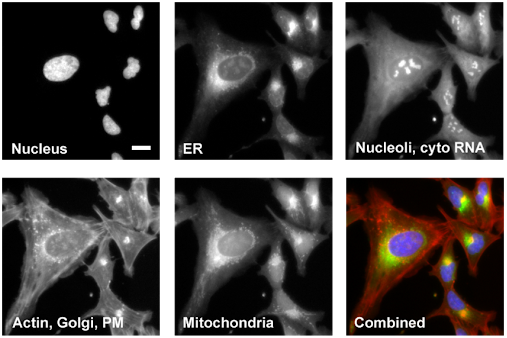
\includegraphics[width=0.98\linewidth,height=0.85\textheight,keepaspectratio]{assets/cell-painting-channels.png}
\end{column}
\end{columns}

\par\smallskip\hfill{\fontsize{5.5}{6.5}\selectfont\color{gray}\href{https://github.com/afermg/2024_10_i2k_poster_flashtalk/blob/bf1db9f818dcc2704bd5ad388c3173a3426f8faf/figs/cellpainting.png}{Source: Muñoz, I2K (2024); assay: Bray et al. (2016)}}
\end{frame}
% END FRAME: sec:org0000001
% BEGIN FRAME: sec:org0000002
\begin{frame}[label={sec:org0000002}]{Cell Painting turns images into measurements}
Profiles are numerical descriptions of cells.

\begin{center}
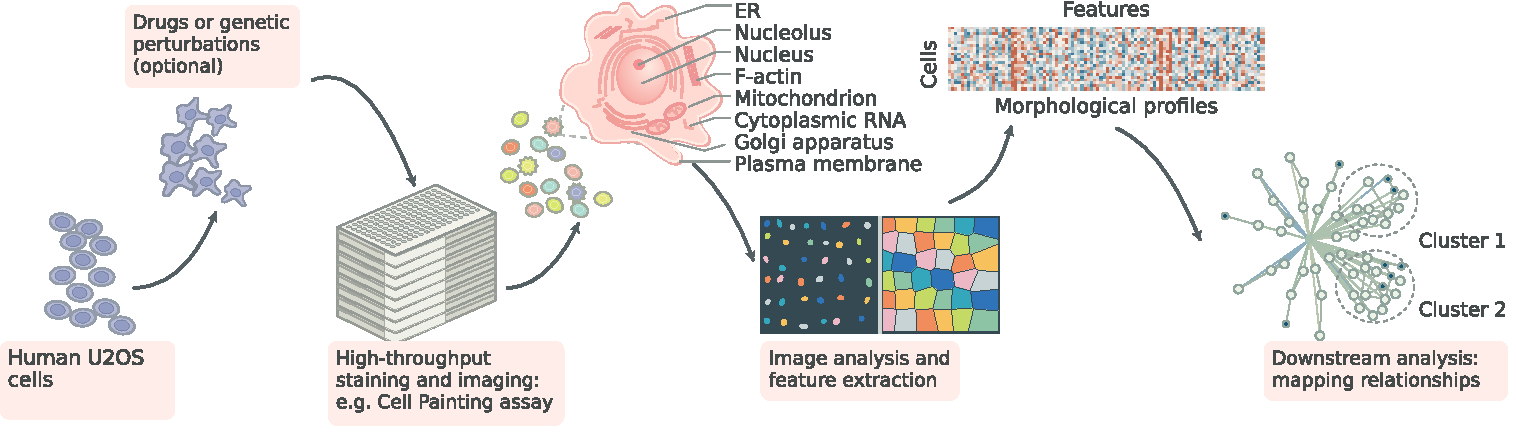
\includegraphics[keepaspectratio,width=0.99\linewidth,height=0.66\textheight]{assets/cell-painting-edited.pdf}
\end{center}

\par\smallskip\hfill{\fontsize{5.5}{6.5}\selectfont\color{gray}\href{https://doi.org/10.1038/s41573-020-00117-w}{Adapted from Chandrasekaran et al. (2021), Fig. 1a}}
\end{frame}
% END FRAME: sec:org0000002
% BEGIN FRAME: sec:org0000006
\begin{frame}[label={sec:org0000006}]{JUMP: Joint Undertaking for Morphological Profiling}
\begin{itemize}
\item Public Cell Painting data: 12 laboratories, around 136,000 perturbations.
\item \href{https://github.com/broadinstitute/jump-profiling-recipe/tree/d2512d978ca17aafead0e99de66386337e6312e4/inputs/cell_counts}{1.8 billion cells}; \textasciitilde{}58.3 million images.
\end{itemize}
\begin{center}
\fbox{\parbox[c][29mm][c]{0.27\linewidth}{\centering CRISPR knockout\par\medskip{\Large\bfseries 7,975}\par gene targets}}
\quad
\fbox{\parbox[c][29mm][c]{0.27\linewidth}{\centering\small Gene overexpression (ORF)\par\smallskip{\Large\bfseries 12,609}\par genes}}
\quad
\fbox{\parbox[c][29mm][c]{0.27\linewidth}{\centering Compound treatment\par\medskip{\Large\bfseries 115,794}\par compounds}}
\end{center}
\end{frame}
% END FRAME: sec:org0000006
% BEGIN FRAME: sec:org0000007
\begin{frame}[label={sec:org0000007}]{We make JUMP accessible via the JUMP Hub}
\begin{columns}[c,onlytextwidth]
\begin{column}{0.60\textwidth}
\centering
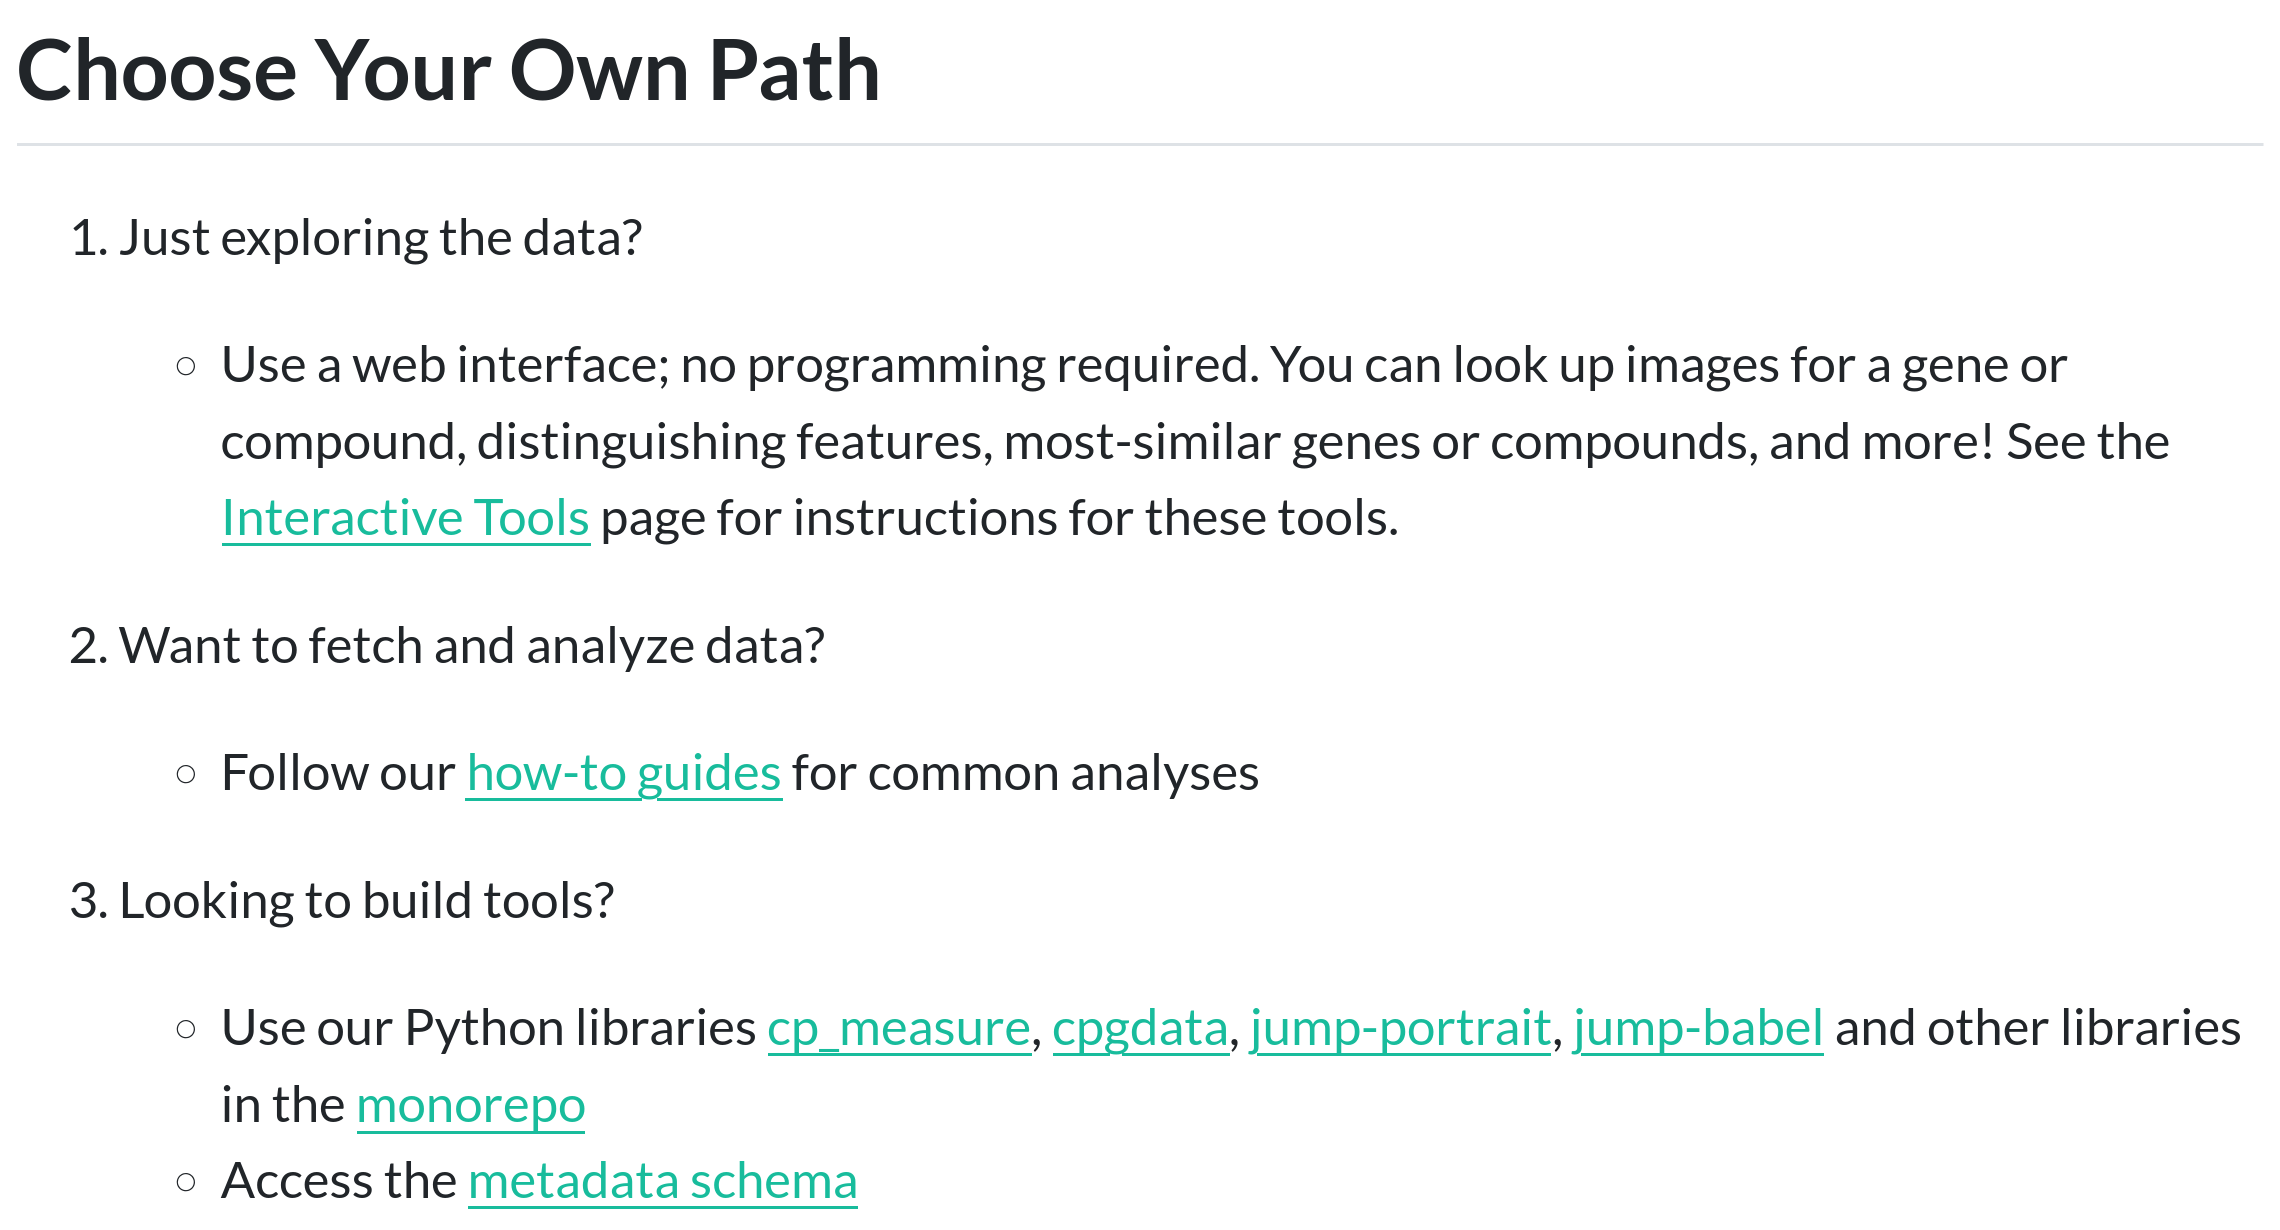
\includegraphics[width=0.98\linewidth,height=0.71\textheight,keepaspectratio]{assets/jump-hub-homepage.png}
\end{column}
\begin{column}{0.37\textwidth}
\textbf{Biologists can find out:}\par\smallskip
\begin{itemize}
\item Does my gene or compound have a phenotype?
\item Which perturbations cause similar phenotypes?
\item What changes in cells and organelles?
\item Is the phenotype heterogeneous across cells/samples?
\end{itemize}
\end{column}
\end{columns}

\par\smallskip\hfill{\fontsize{5.5}{6.5}\selectfont\color{gray}\href{https://broadinstitute.github.io/jump_hub/}{Source: JUMP Hub (2026)}}
\end{frame}
% END FRAME: sec:org0000007



% BEGIN FRAME: sec:org0000008
\begin{frame}[label={sec:org0000008}]{Tutorials, how-tos and resources}
The Hub contains practical guides to help biologists use JUMP.

\medskip
\begin{tabular}{@{}>{\raggedright\arraybackslash}p{0.27\textwidth}>{\raggedright\arraybackslash}p{0.68\textwidth}@{}}
\textbf{How-to guides} & \href{https://broadinstitute.github.io/jump_hub/howto/interactive/1_jumprr_steps.html}{No-code gene/compound queries}; \href{https://broadinstitute.github.io/jump_hub/howto/interactive/0_overview.html\#morpheus}{explore similarity heatmaps}. \\[1em]
\textbf{Tutorials} & \href{https://broadinstitute.github.io/jump_hub/howto/notebooks/0_overview.html}{Curated runnable notebooks for profiles, metadata and statistical analysis.} \\[1em]
\textbf{Further resources} & \href{https://broadinstitute.github.io/jump_hub/explanations/data_description.html}{Dataset explanations}, \href{https://broadinstitute.github.io/jump_hub/howto/notebooks/17_mislocus_example.html}{protein-localisation analysis} and a \href{https://ciminilab.github.io/GuideToCellPainting/}{Guide to Cell Painting for Biologists}.
\end{tabular}\par\bigskip
\end{frame}
% END FRAME: sec:org0000008
\section*{From the literature to a JUMP workflow}
% Shared Org/TeX sequence: OPA1 and DNM1L, raw JUMP images and AI-assisted interfaces.
% Exact source fields, display limits and crop rule: docs/gene-examples-provenance.json.
% BEGIN FRAME: sec:org0000009
\begin{frame}[label={sec:org0000009}]{A tale of two genes (that shape mitochondria)}
\begin{columns}[T,onlytextwidth]
\begin{column}{0.47\textwidth}
\textbf{OPA1: mitochondrial fusion}
\begin{itemize}
\item Helps mitochondria fuse.
\item Loss is expected to produce shorter, fragmented networks.
\end{itemize}
\end{column}
\begin{column}{0.47\textwidth}
\textbf{DNM1L / DRP1: mitochondrial division}
\begin{itemize}
\item Helps mitochondria divide.
\item Loss is expected to produce longer, more-connected networks.
\end{itemize}
\end{column}
\end{columns}
\bigskip
\textbf{Can we validate the phenotypes using our high-throughput methods?}
\par\bigskip
{\scriptsize From \href{https://doi.org/10.1083/jcb.200704112}{Griparic et al., JCB (2007), Fig. 3}; \href{https://doi.org/10.1091/mbc.12.8.2245}{Smirnova et al., MBoC (2001)}.}
\end{frame}
% END FRAME: sec:org0000009

% BEGIN FRAME: literature:opa1-siRNA
\begin{frame}[label={literature:opa1-siRNA}]{OPA1 depletion fragments mitochondria}
\begin{columns}[c,onlytextwidth]
\begin{column}{0.48\textwidth}
\centering\textbf{OPA1 siRNA}\par\smallskip
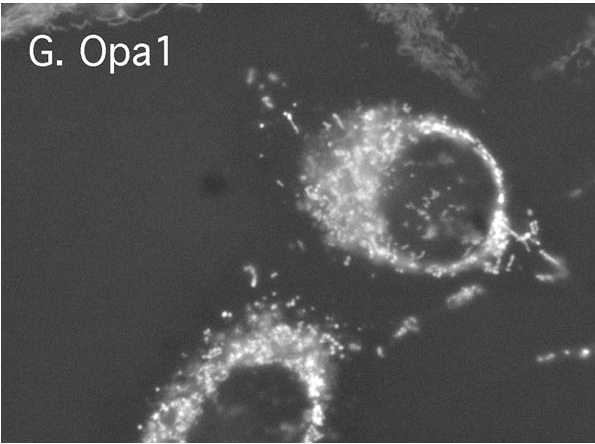
\includegraphics[width=0.96\linewidth,height=0.57\textheight,keepaspectratio]{assets/opa1-literature/OPA1-siRNA-panel-G.png}
\end{column}
\begin{column}{0.48\textwidth}
\centering\textbf{Scrambled siRNA}\par\smallskip
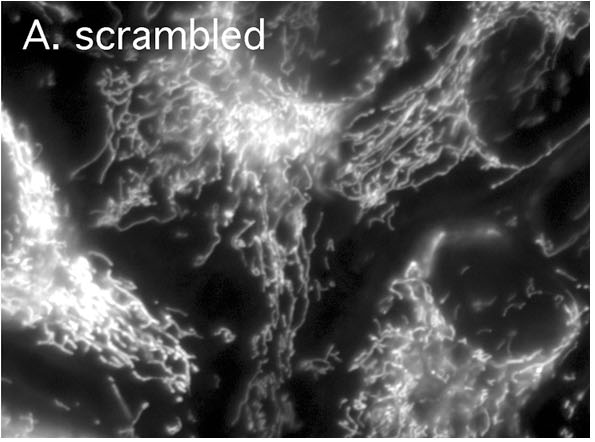
\includegraphics[width=0.96\linewidth,height=0.57\textheight,keepaspectratio]{assets/opa1-literature/control-siRNA-panel-A.png}
\end{column}
\end{columns}
\medskip
{\small HeLa cells; MitoTracker. OPA1 depletion for 2 days.}
\par\medskip
{\scriptsize\href{https://doi.org/10.1083/jcb.200704112}{Griparic, Kanazawa \& van der Bliek, JCB (2007), Fig. 3G/A}. cropped}
\end{frame}
% END FRAME: literature:opa1-siRNA

% BEGIN FRAME: literature:dnm1l-siRNA
\begin{frame}[label={literature:dnm1l-siRNA}]{DRP1 depletion increases connectivity}
\begin{columns}[c,onlytextwidth]
\begin{column}{0.48\textwidth}
\centering\textbf{DNM1L / DRP1 siRNA}\par\smallskip
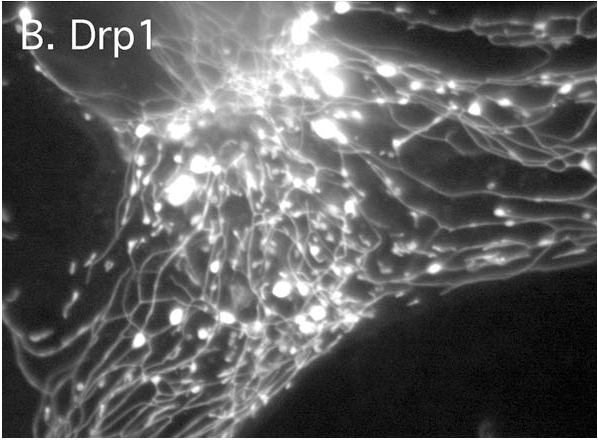
\includegraphics[width=0.96\linewidth,height=0.57\textheight,keepaspectratio]{assets/opa1-literature/DRP1-siRNA-panel-B.png}
\end{column}
\begin{column}{0.48\textwidth}
\centering\textbf{Scrambled siRNA}\par\smallskip
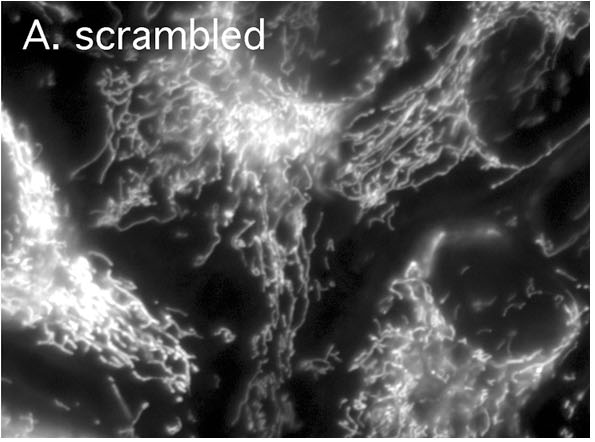
\includegraphics[width=0.96\linewidth,height=0.57\textheight,keepaspectratio]{assets/opa1-literature/control-siRNA-panel-A.png}
\end{column}
\end{columns}
\medskip
{\small HeLa cells; MitoTracker. DRP1 depletion for 2 days.}
\par\medskip
{\scriptsize\href{https://doi.org/10.1083/jcb.200704112}{Griparic, Kanazawa \& van der Bliek, JCB (2007), Fig. 3B/A}. Published microscopy, cropped.}
\end{frame}
% END FRAME: literature:dnm1l-siRNA

% BEGIN FRAME: sec:org000000d
\begin{frame}[label={sec:org000000d}]{Where to start?}
\textbf{Find the perturbations for OPA1 and DNM1L.}\par\bigskip
\begin{itemize}
\item Start with the gallery and find matching negative controls.
\item Look it up in our available tables.
\item Find related perturbations through profile similarity.
\end{itemize}
\bigskip
{\scriptsize\href{https://broadinstitute.github.io/jump_hub/reference/00_gene_index.html}{JUMP Hub gene availability}}
\end{frame}
% END FRAME: sec:org000000d

% BEGIN FRAME: tutorial:availability
\begin{frame}[label={tutorial:availability}]{Is the gene represented in JUMP?}
\centering
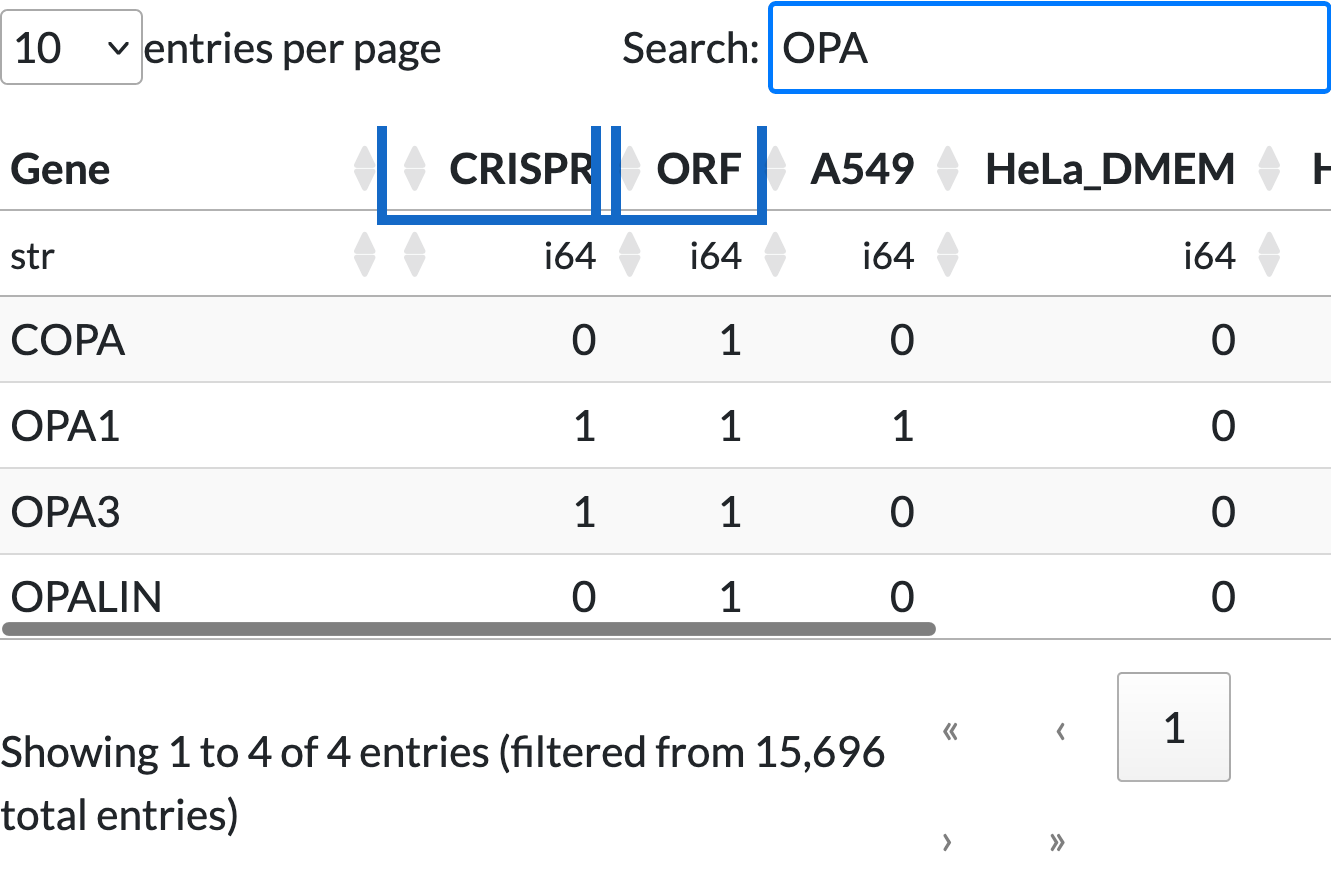
\includegraphics[width=0.98\linewidth,height=0.72\textheight,keepaspectratio]{assets/opa1-tutorial-screenshots/01-availability.png}
\par\medskip
{\footnotesize\raggedright\textbf{How:} search OPA, identify OPA1 among the returned genes, and check which CRISPR and ORF perturbations we can follow into the feature tables.\par}
% Published JUMP_rr coverage row; see docs/opa1-tutorial-screenshots-provenance.json.
\end{frame}
% END FRAME: tutorial:availability

% BEGIN FRAME: sec:org0000010
\begin{frame}[label={sec:org0000010}]{How do the cells look?}
\centering
{\small\textbf{CRISPR Gallery --- OPA1}}\par\smallskip
\includegraphics[width=0.98\linewidth,height=0.65\textheight,keepaspectratio]{assets/opa1-tutorial-screenshots/00-opa1-crispr-gallery.png}
\par\smallskip
{\scriptsize\raggedright\textbf{Tip:} enlarge image previews on hover with \href{https://addons.mozilla.org/en-US/firefox/addon/imagus/}{Imagus (Firefox)} or \href{https://chromewebstore.google.com/detail/hover-zoom\%2B/pccckmaobkjjboncdfnnofkonhgpceea}{Hover Zoom+ (Chrome)}.\par}
\end{frame}
% END FRAME: sec:org0000010

% BEGIN FRAME: filtering_example
\begin{frame}[label={filtering_example}]{Filtering example: one OPA1 well}
\centering
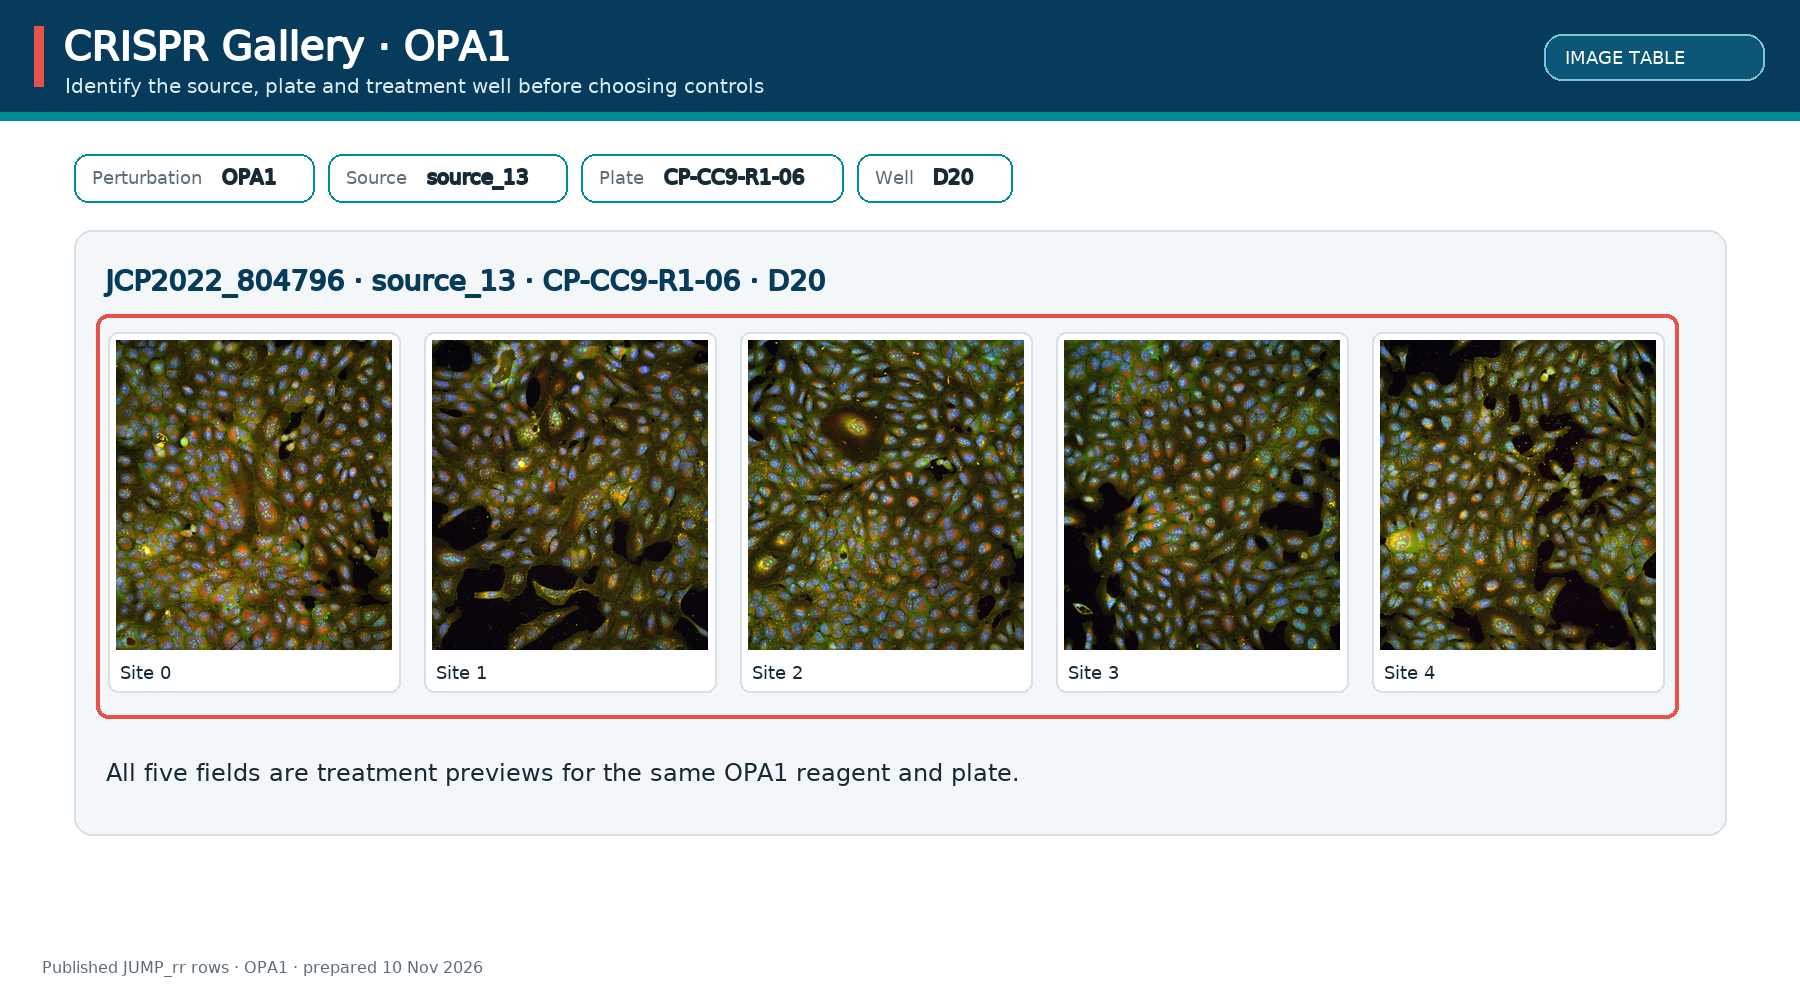
\includegraphics[trim=0 200bp 300bp 0,clip,width=0.98\linewidth,height=0.72\textheight,keepaspectratio]{assets/opa1-tutorial-screenshots/04-gallery-perturbation.png}
\par\medskip
{\footnotesize\raggedright\textbf{How:} filter the image table for OPA1, then record source\_13, plate CP-CC9-R1-06 and treatment well D20 before selecting controls.\par}
% Published JUMP_rr OPA1 CRISPR gallery row and preview images; see provenance JSON.
\end{frame}
% END FRAME: filtering_example
% BEGIN FRAME: tutorial:gallery-controls
\begin{frame}[label={tutorial:gallery-controls}]{What should we compare those cells against?}
\centering
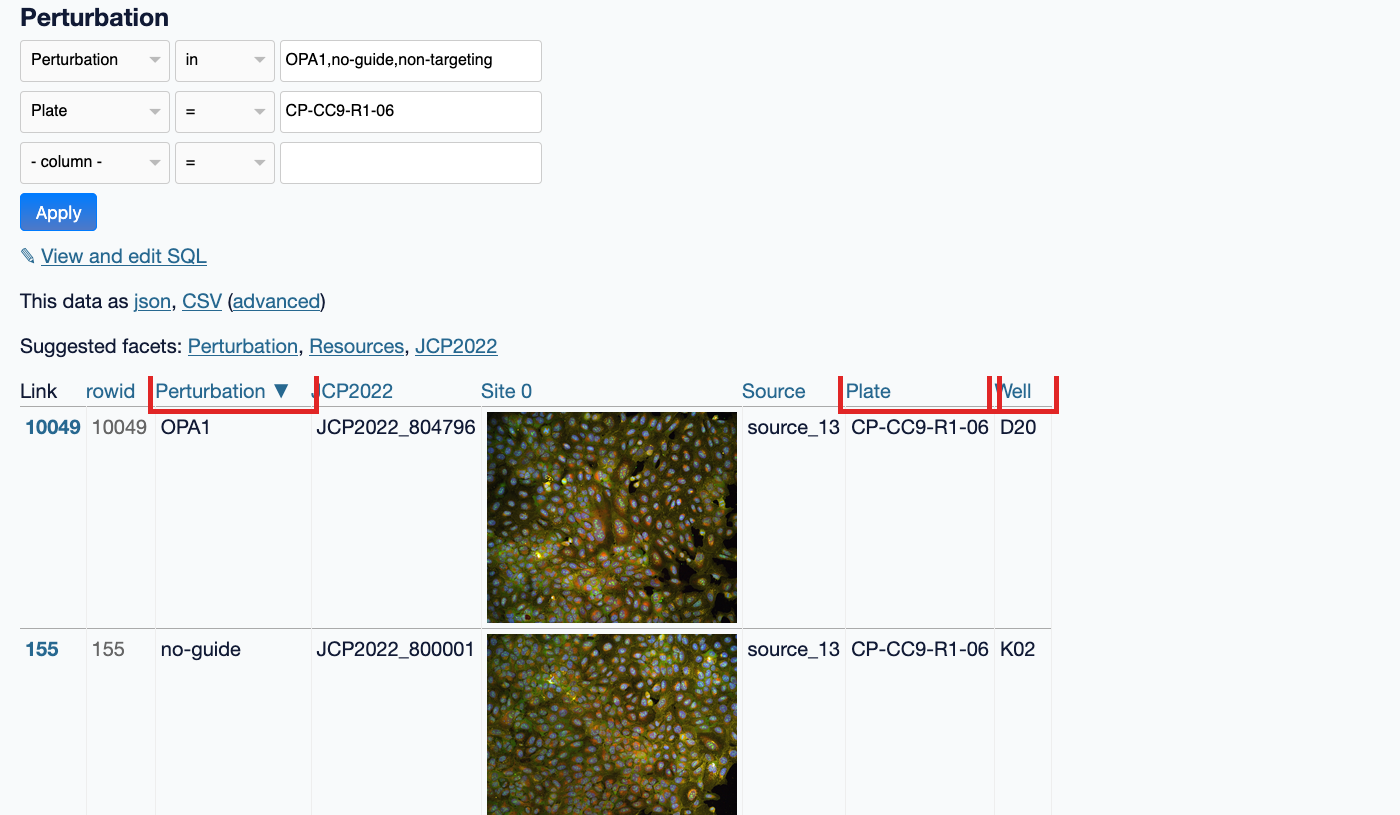
\includegraphics[trim=0 0 300bp 260bp,clip,width=0.98\linewidth,height=0.72\textheight,keepaspectratio]{assets/opa1-tutorial-screenshots/05-gallery-controls.png}
\par\medskip
{\footnotesize\raggedright\textbf{How:} retain source\_13 and CP-CC9-R1-06, then add no-guide and non-targeting controls from that same plate.\par}
% Published JUMP_rr OPA1 and control gallery rows and preview images; see provenance JSON.
\end{frame}
% END FRAME: tutorial:gallery-controls
% BEGIN FRAME: tutorial:interface
\begin{frame}[label={tutorial:interface}]{Which table columns answer our question?}
\centering
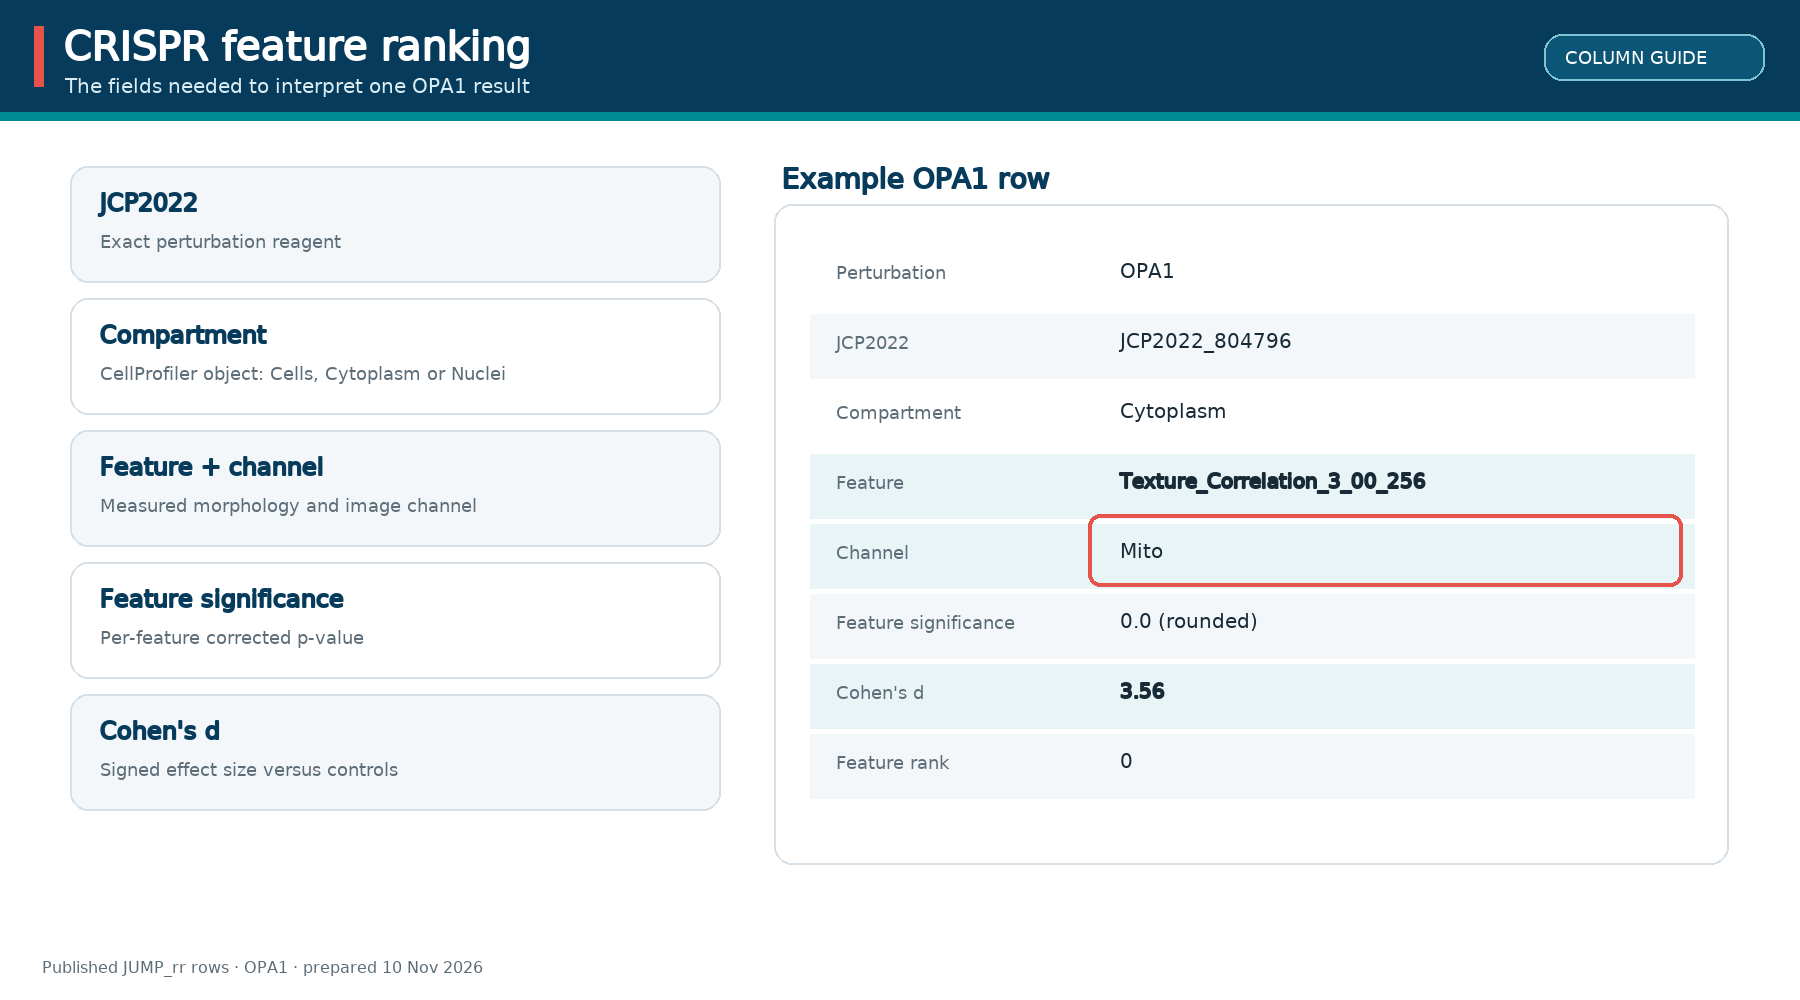
\includegraphics[trim=10bp 175bp 10bp 225bp,clip,width=0.98\linewidth,height=0.72\textheight,keepaspectratio]{assets/opa1-tutorial-screenshots/02-columns.png}
\par\medskip
{\footnotesize\raggedright\textbf{How:} read the OPA1 row's reagent, compartment, feature, channel, per-feature significance and signed effect size.\par}
% Published JUMP_rr OPA1 CRISPR feature row; see provenance JSON.
\end{frame}
% END FRAME: tutorial:interface
% BEGIN FRAME: tutorial:filters
\begin{frame}[label={tutorial:filters}]{How do we isolate the gene we care about?}
\centering
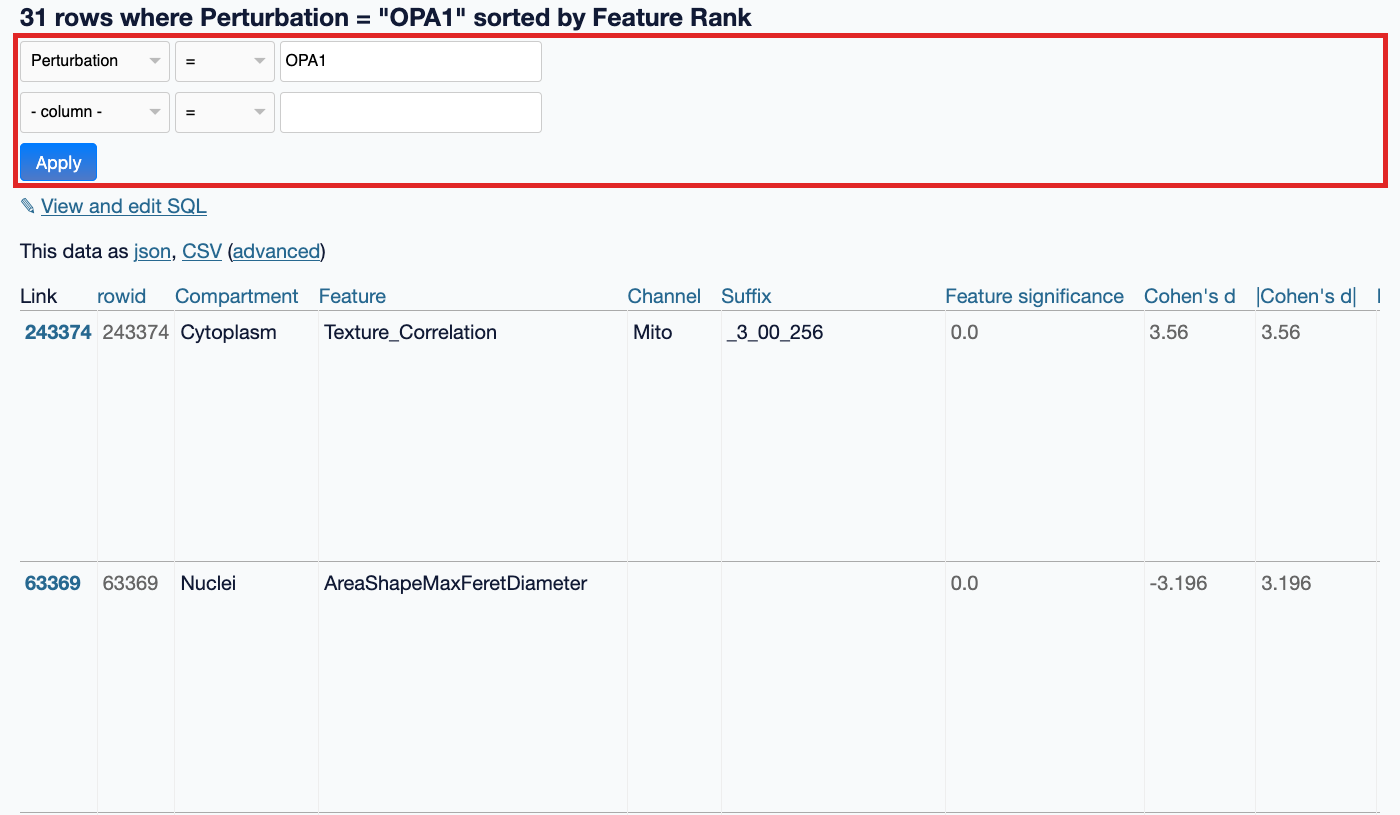
\includegraphics[trim=0 250bp 0 0,clip,width=0.98\linewidth,height=0.72\textheight,keepaspectratio]{assets/opa1-tutorial-screenshots/03-filters.png}
\par\medskip
{\footnotesize\raggedright\textbf{How:} filter by the exact symbol OPA1 or a published synonym such as MGM1, then add object-level filters when needed.\par}
% Published JUMP_rr OPA1 rows and synonyms; see provenance JSON.
\end{frame}
% END FRAME: tutorial:filters
% BEGIN FRAME: tutorial:activity
\begin{frame}[label={tutorial:activity}]{Does the perturbation have a measurable phenotype?}
\centering
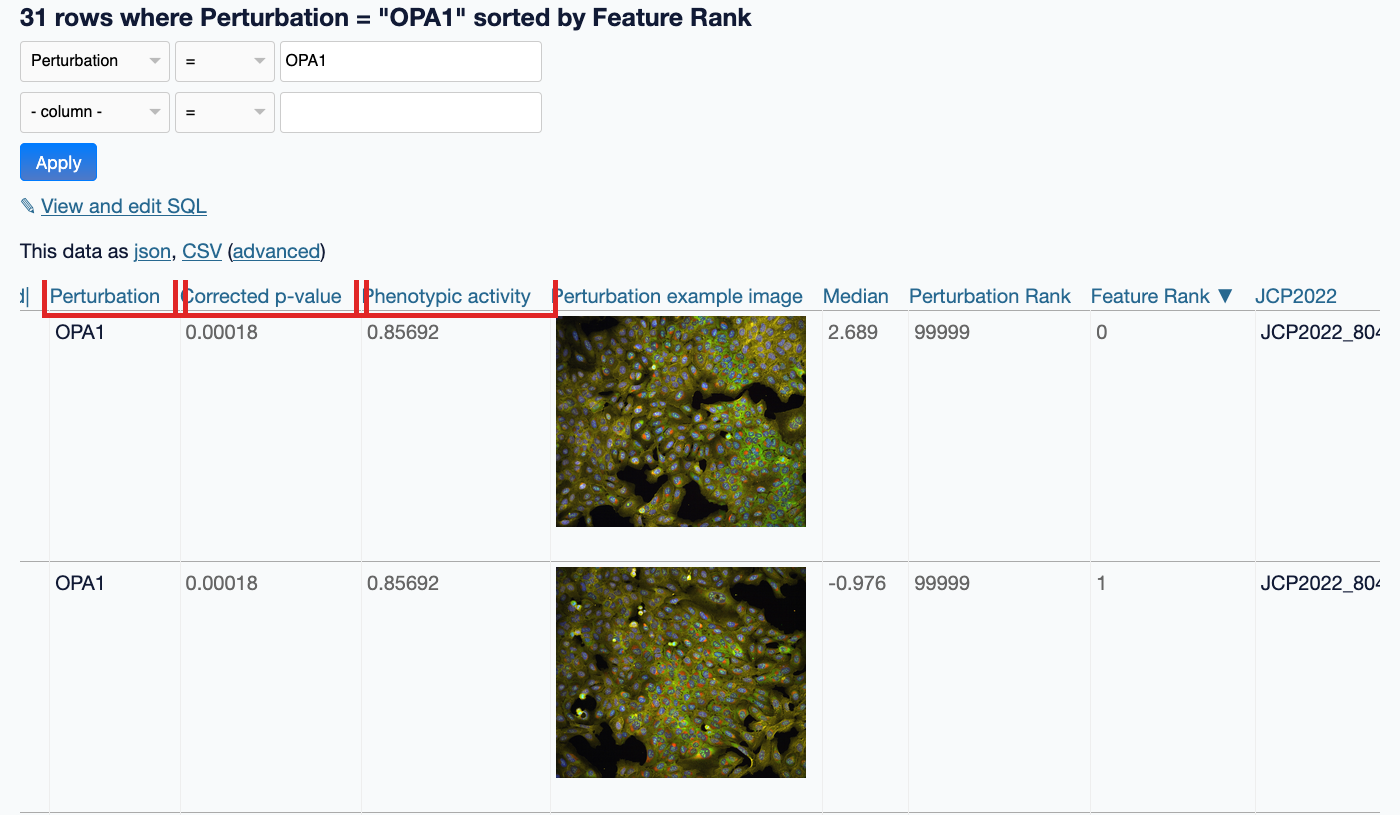
\includegraphics[trim=0 250bp 0 0,clip,width=0.98\linewidth,height=0.72\textheight,keepaspectratio]{assets/opa1-tutorial-screenshots/06-activity.png}
\par\medskip
{\footnotesize\raggedright\textbf{How:} read the perturbation-level values: OPA1 CRISPR $p=0.00018$, activity $0.85692$; OPA1 ORF $p=0.03371$, activity $0.70875$.\par}
% Published JUMP_rr OPA1 CRISPR and ORF rows; see provenance JSON.
\end{frame}
% END FRAME: tutorial:activity
% BEGIN FRAME: tutorial:rows
\begin{frame}[label={tutorial:rows}]{What does one feature result describe?}
\centering
{\small\textbf{OPA1 CRISPR: one feature, read across two close-ups}}\par\medskip
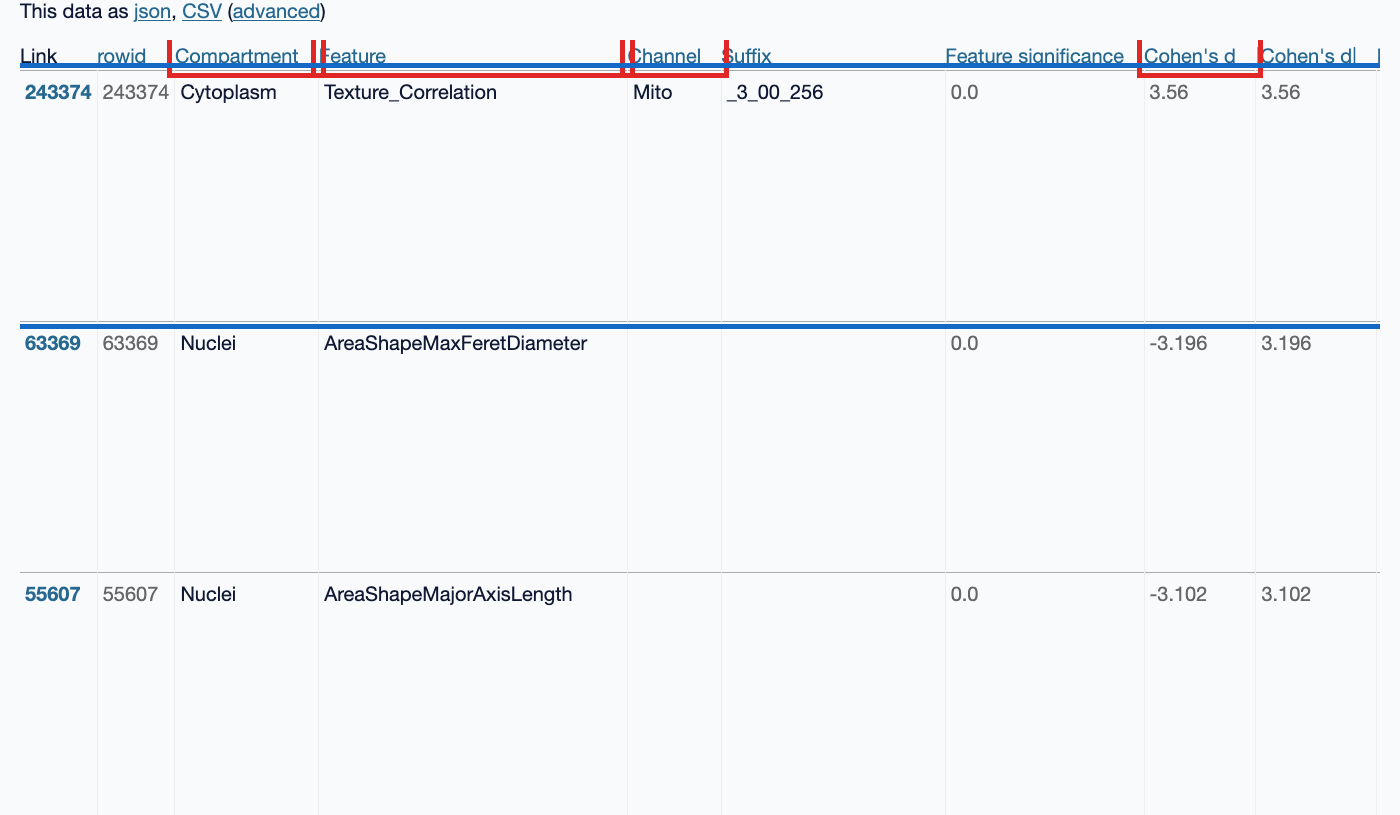
\includegraphics[trim=175bp 700bp 680bp 40bp,clip,width=0.92\linewidth]{assets/opa1-tutorial-screenshots/07-feature-row.png}\par\bigskip
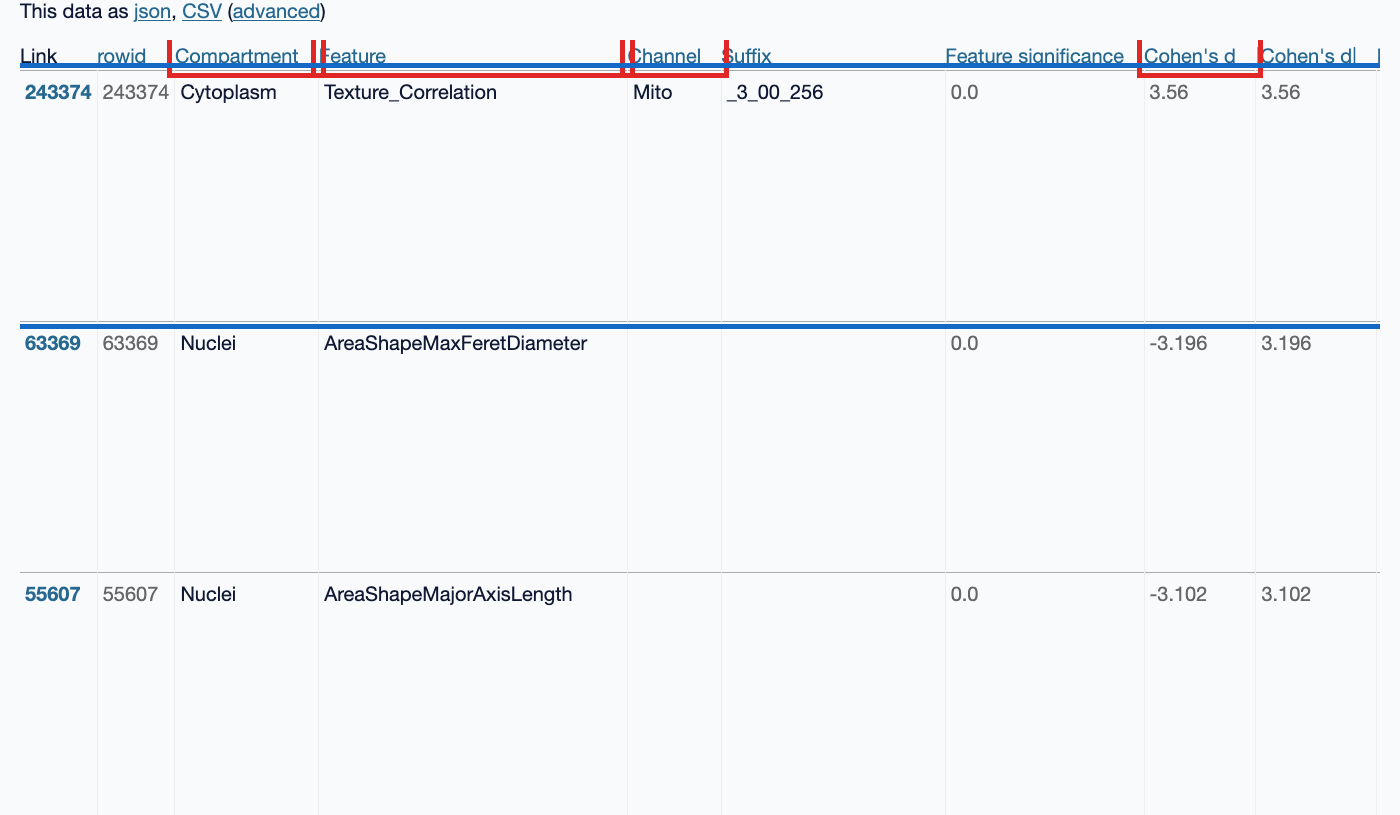
\includegraphics[trim=720bp 700bp 150bp 40bp,clip,width=0.92\linewidth]{assets/opa1-tutorial-screenshots/07-feature-row.png}
\par\medskip
{\footnotesize\raggedright\textbf{How:} read across one OPA1 row: reagent, object, feature, channel, significance, effect size and rank. It summarizes a profile, not one cell.\par}
% Published JUMP_rr OPA1 CRISPR feature row; see provenance JSON.
\end{frame}
% END FRAME: tutorial:rows
% BEGIN FRAME: tutorial:features
\begin{frame}[label={tutorial:features}]{Which features explain the differences?}
\centering
{\small\textbf{OPA1 CRISPR: the top-ranked feature}}\par\medskip
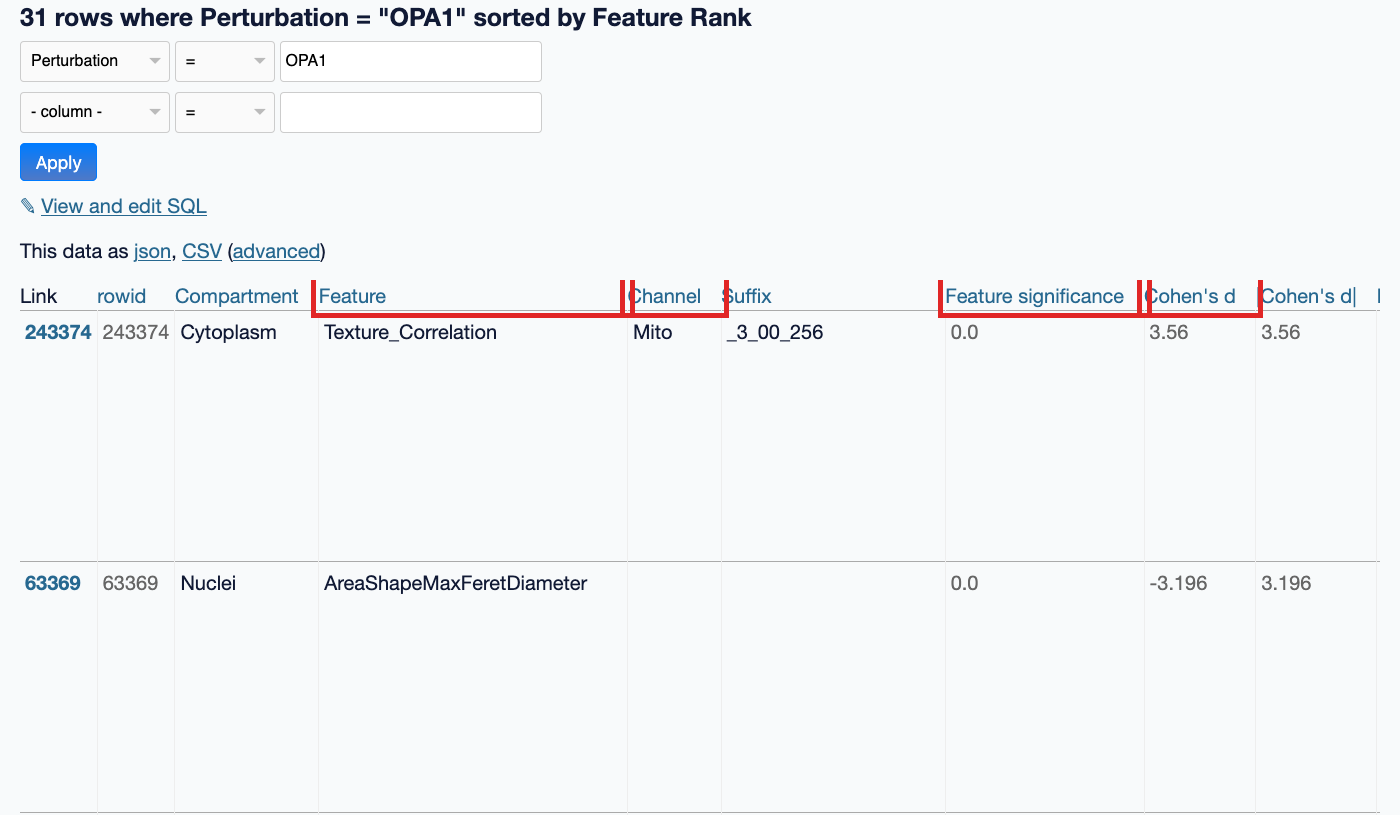
\includegraphics[trim=175bp 456bp 680bp 282.5bp,clip,width=0.92\linewidth]{assets/opa1-tutorial-screenshots/08-crispr-features.png}\par\bigskip
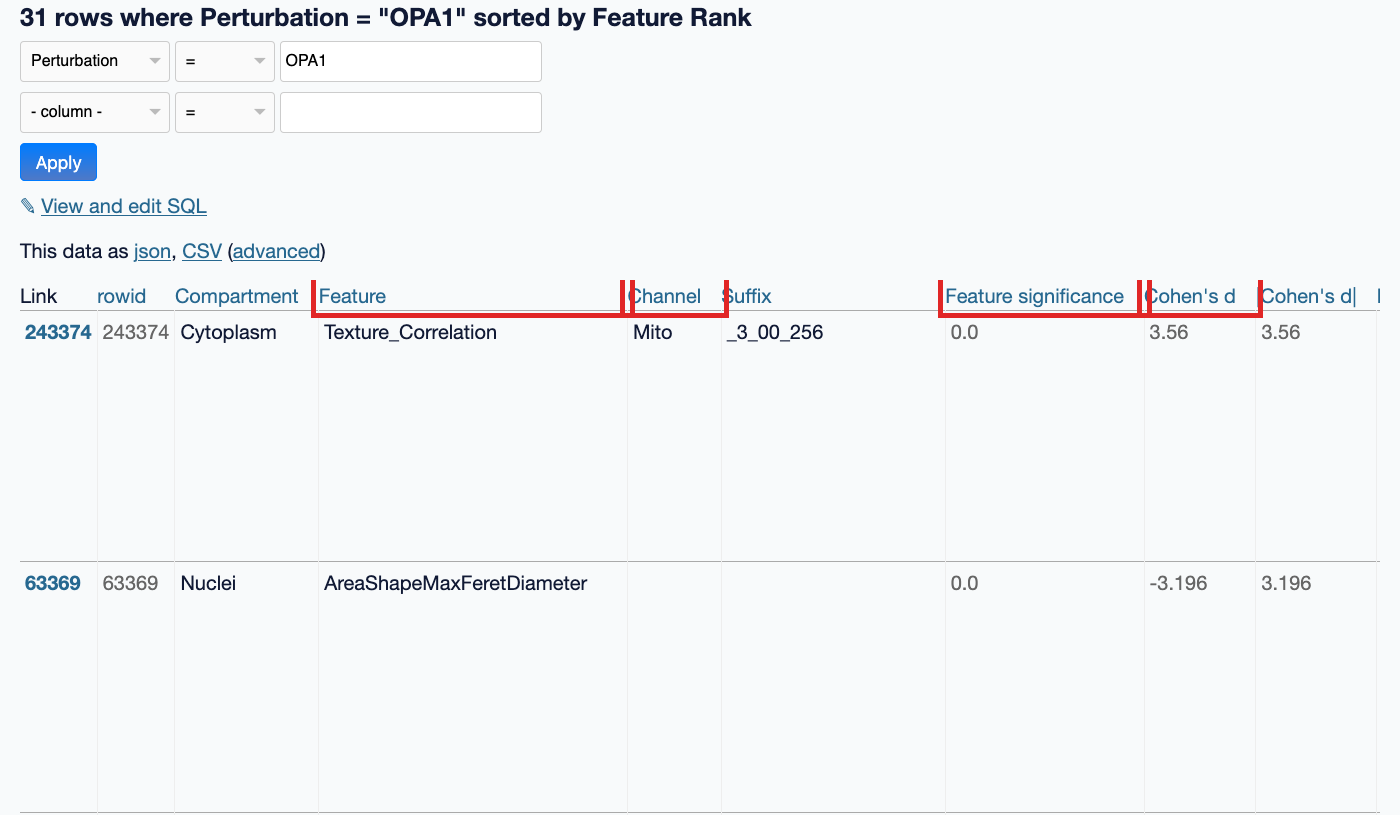
\includegraphics[trim=720bp 456bp 150bp 282.5bp,clip,width=0.92\linewidth]{assets/opa1-tutorial-screenshots/08-crispr-features.png}
\par\medskip
{\footnotesize\raggedright\textbf{How:} sort OPA1 CRISPR rows by feature rank and compare significance with signed effect size; the leading row is a Mito texture feature.\par}
% Published JUMP_rr OPA1 CRISPR feature rows; see provenance JSON.
\end{frame}
% END FRAME: tutorial:features

% BEGIN FRAME: sec:org000000c
\begin{frame}[label={sec:org000000c}]{CellProfiler detects mitochondrial feature changes}
\begin{tabular}{@{}l l r@{}}
\textbf{Gene} & \textbf{Feature} & \textbf{Cohen's $d$} \\[8pt]
OPA1 & Mito texture correlation & $+3.56$ \\[6pt]
DNM1L & Mito-skeleton branch ends & $-5.95$ \\[6pt]
DNM1L & Mito granularity & $+4.09$ \\[6pt]
DNM1L & Mito-skeleton total length & $-3.55$
\end{tabular}
\par\bigskip
\textbf{Mitochondrial organization changes.}
\end{frame}
% END FRAME: sec:org000000c

% BEGIN FRAME: tutorial:orf
\begin{frame}[label={tutorial:orf}]{What happens with a different perturbation type?}
\centering
{\small\textbf{OPA1 ORF: a separate perturbation and feature ranking}}\par\medskip
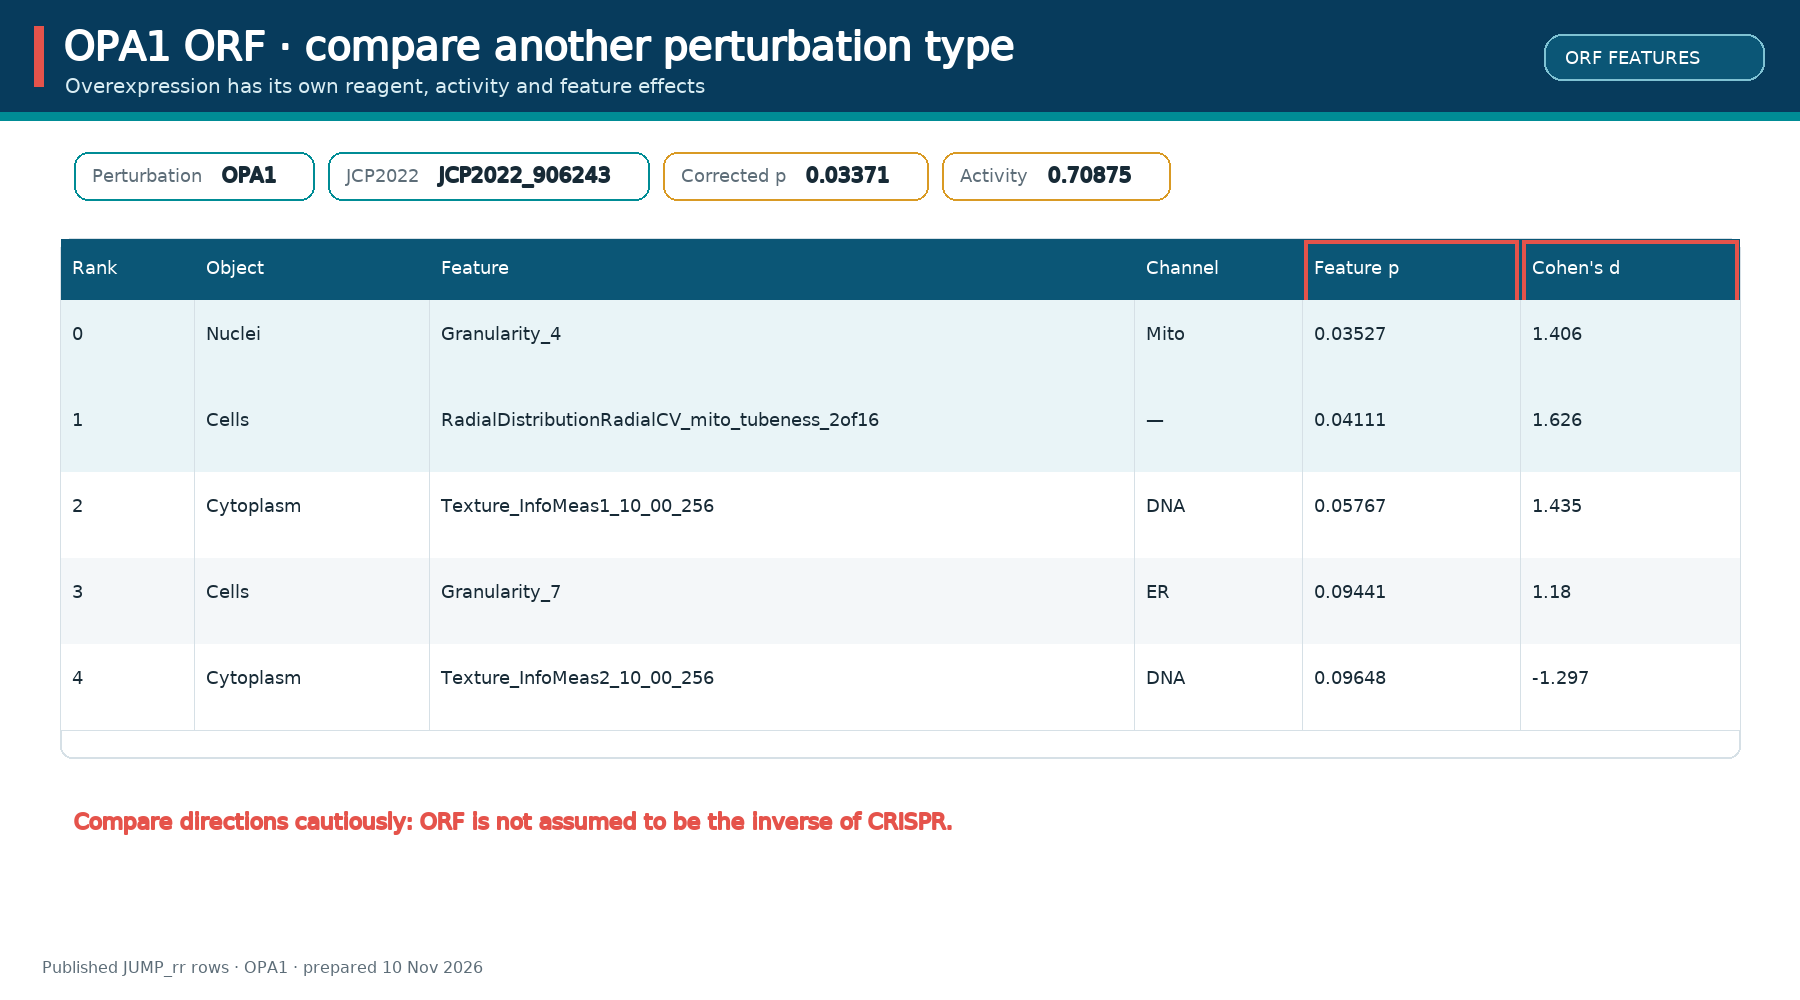
\includegraphics[trim=175bp 456bp 700bp 282.5bp,clip,width=0.92\linewidth]{assets/opa1-tutorial-screenshots/09-orf-features.png}\par\bigskip
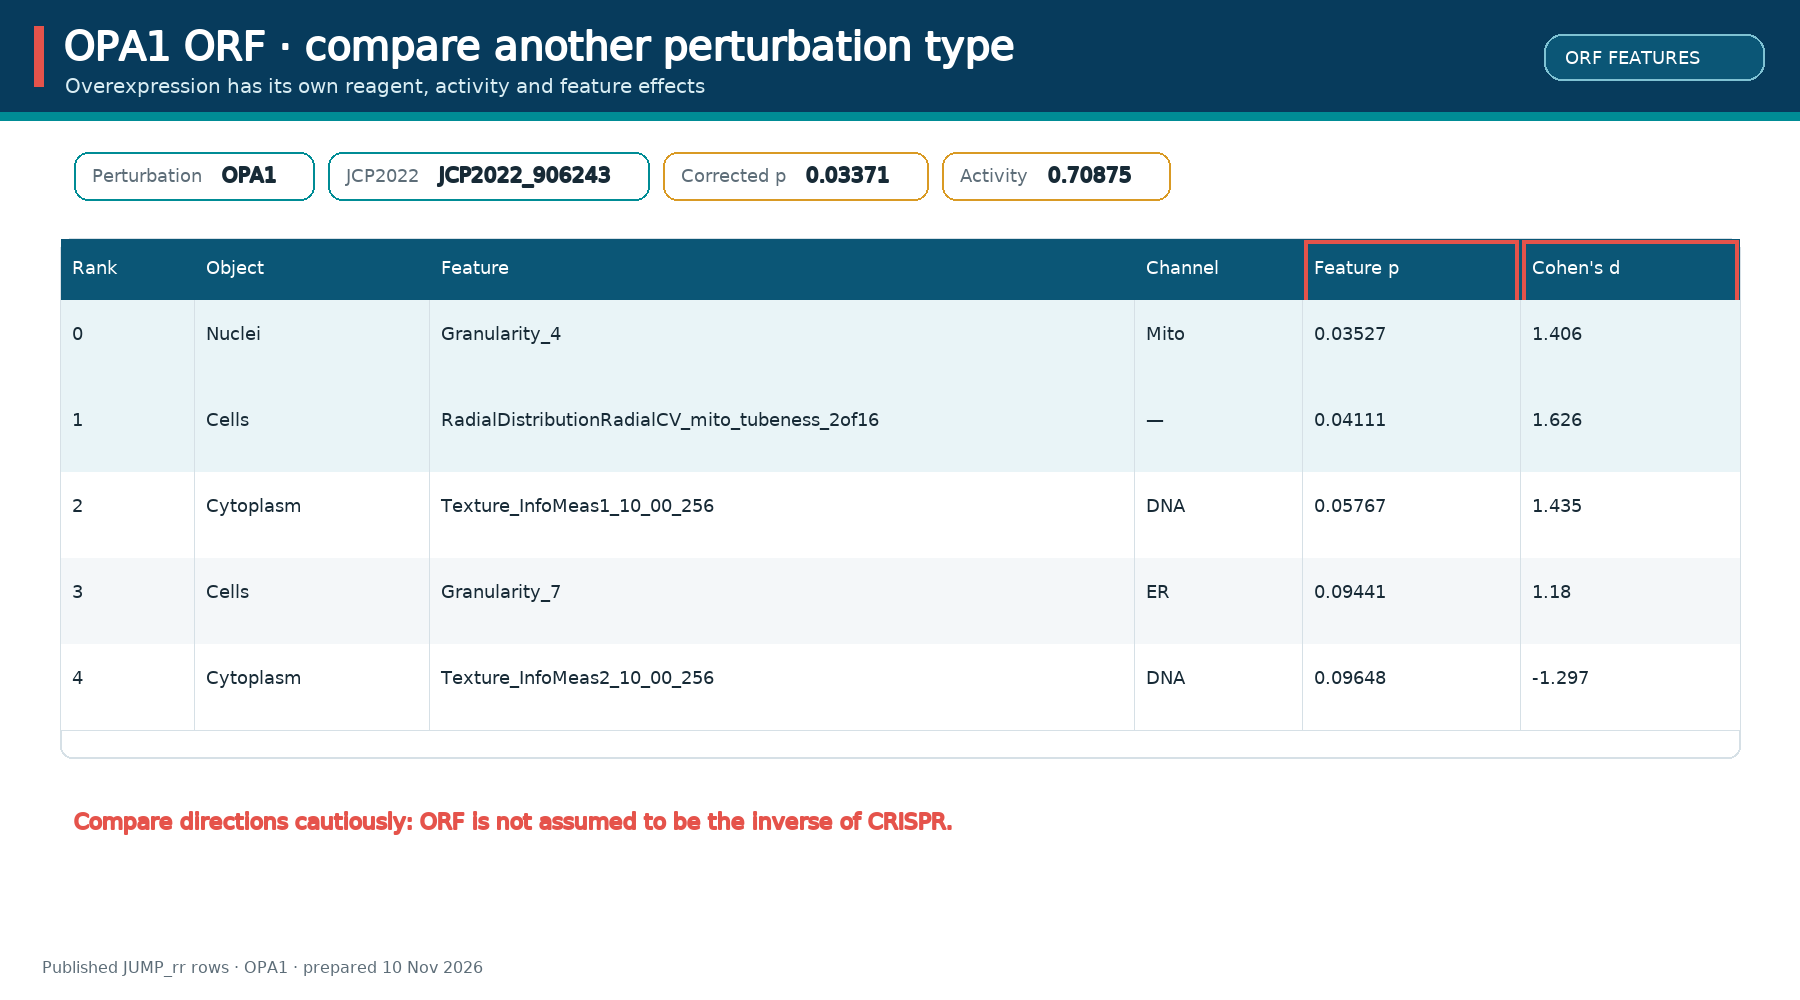
\includegraphics[trim=920bp 456bp 175bp 282.5bp,clip,width=0.65\linewidth]{assets/opa1-tutorial-screenshots/09-orf-features.png}
\par\medskip
{\footnotesize\raggedright\textbf{How:} open OPA1 in the ORF table and compare its separate reagent, activity and ranked feature effects with CRISPR.\par}
% Published JUMP_rr OPA1 ORF feature rows; see provenance JSON.
\end{frame}
% END FRAME: tutorial:orf
% BEGIN FRAME: tutorial:matches
\begin{frame}[label={tutorial:matches}]{Which other perturbations have similar profiles?}
\centering
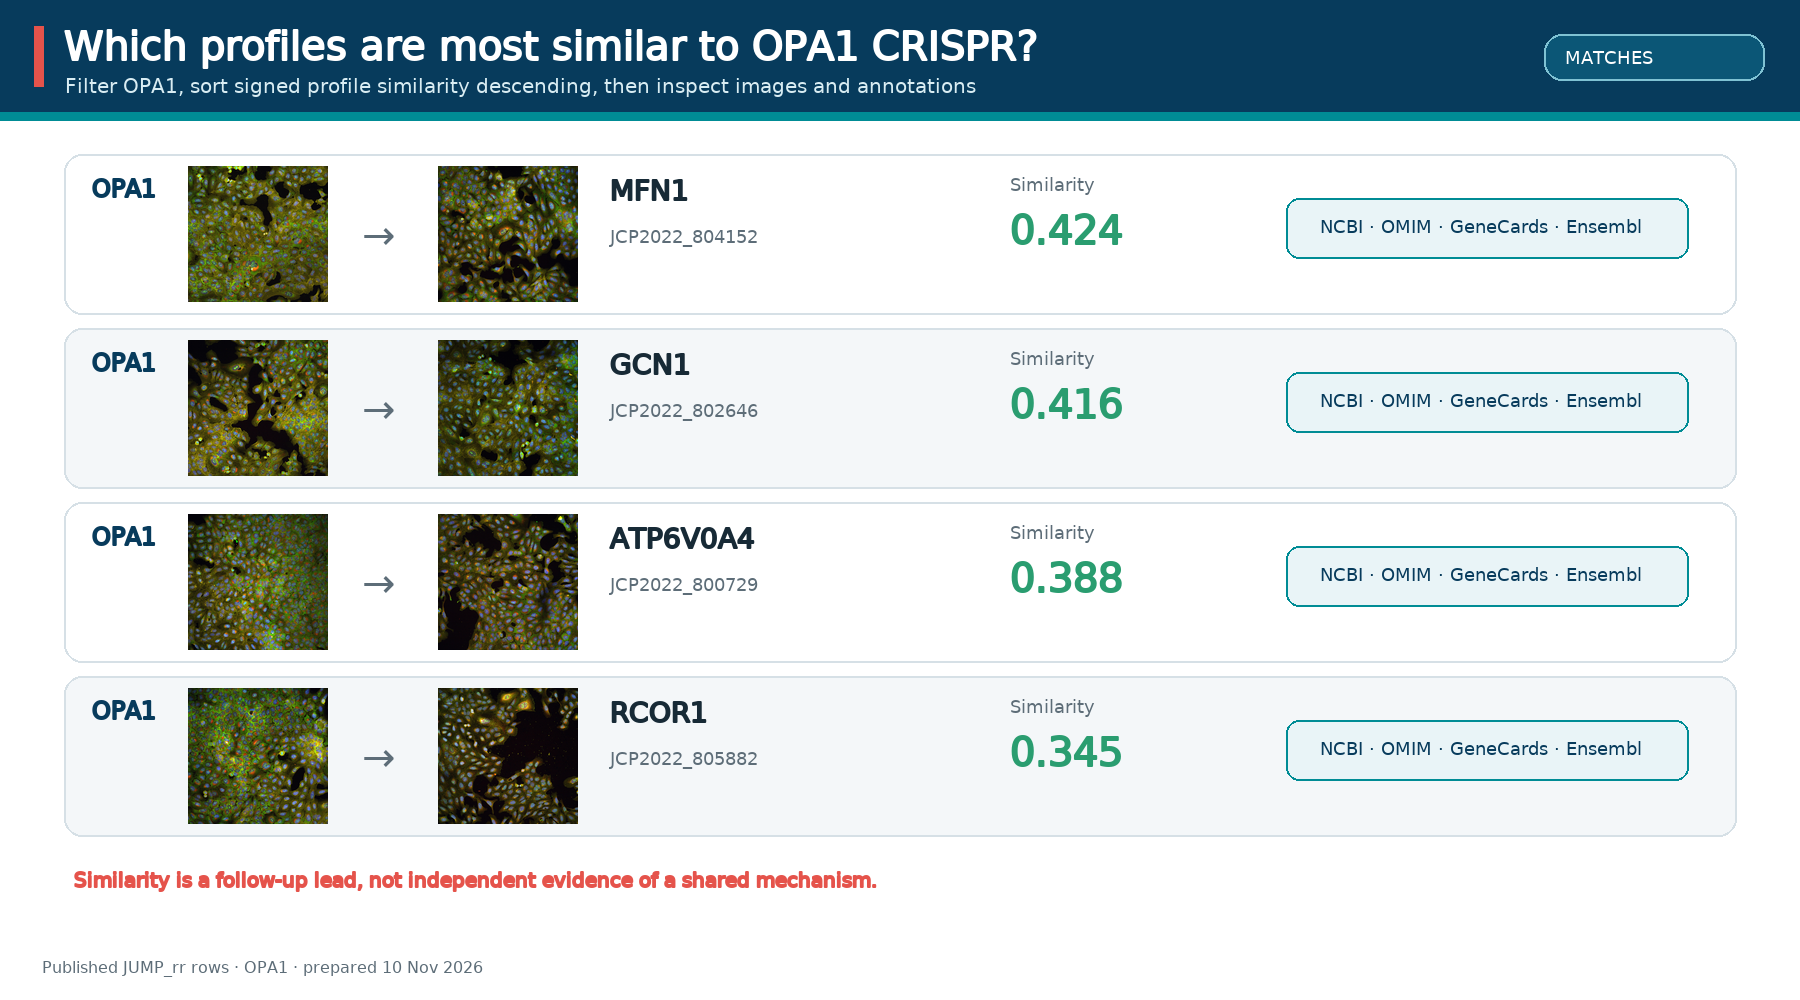
\includegraphics[trim=0 250bp 0 0,clip,width=0.98\linewidth,height=0.72\textheight,keepaspectratio]{assets/opa1-tutorial-screenshots/10-matches.png}
\par\medskip
{\footnotesize\raggedright\textbf{How:} filter the CRISPR match table for OPA1 and sort similarity descending; MFN1 is the strongest published match shown ($0.424$).\par}
% Published JUMP_rr OPA1 CRISPR match rows and preview images; see provenance JSON.
\end{frame}
% END FRAME: tutorial:matches
% BEGIN FRAME: tutorial:export
\begin{frame}[label={tutorial:export}]{How do we keep and share the result?}
\centering
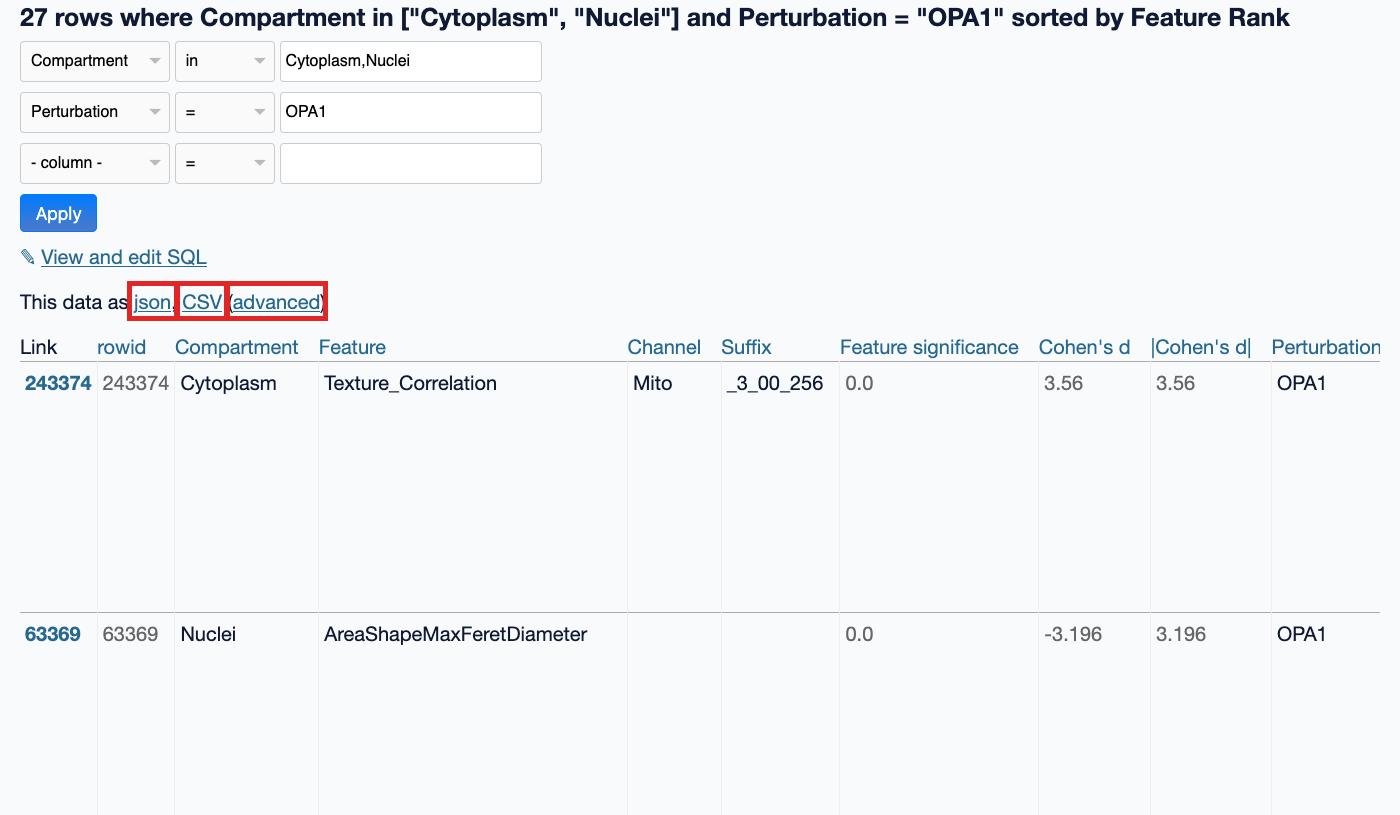
\includegraphics[trim=10bp 495bp 840bp 35bp,clip,width=0.98\linewidth,height=0.66\textheight,keepaspectratio]{assets/opa1-tutorial-screenshots/11-export.png}
\par\medskip
{\footnotesize\raggedright\textbf{How:} keep OPA1 and the relevant objects, then export the rows with the reagent ID, filters and source URL.\par}
% Published JUMP_rr OPA1 CRISPR feature rows; see provenance JSON.
\end{frame}
% END FRAME: tutorial:export

% BEGIN FRAME: sec:org000000a
\begin{frame}[label={sec:org000000a}]{JUMP example: OPA1 knockout}
\begin{columns}[c,onlytextwidth]
\begin{column}{0.48\textwidth}
\centering\textbf{OPA1 CRISPR knockout}\par\smallskip
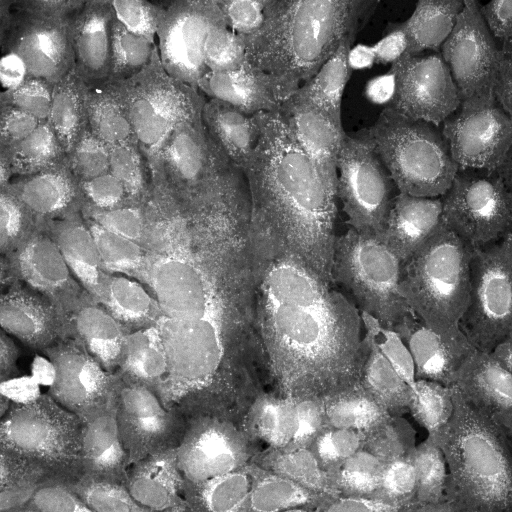
\includegraphics[width=0.92\linewidth,height=0.61\textheight,keepaspectratio]{assets/gene-examples/OPA1-treatment-center512.png}
\end{column}
\begin{column}{0.48\textwidth}
\centering\textbf{No-guide negative control}\par\smallskip
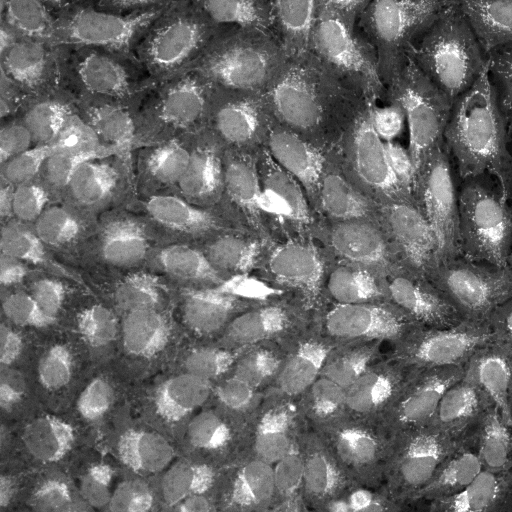
\includegraphics[width=0.92\linewidth,height=0.61\textheight,keepaspectratio]{assets/gene-examples/OPA1-control-center512.png}
\end{column}
\end{columns}
\smallskip
{\scriptsize JUMP Mito channel; source\_13, CP-CC9-R1-06, D20 / B02, field index 0.\\
Both panels share intensity limits 219--3985. \href{https://github.com/jump-cellpainting/datasets}{JUMP data}.}
\end{frame}
% END FRAME: sec:org000000a

% BEGIN FRAME: sec:org000000b
\begin{frame}[label={sec:org000000b}]{JUMP example: DNM1L knockout}
\begin{columns}[c,onlytextwidth]
\begin{column}{0.48\textwidth}
\centering\textbf{DNM1L CRISPR knockout}\par\smallskip
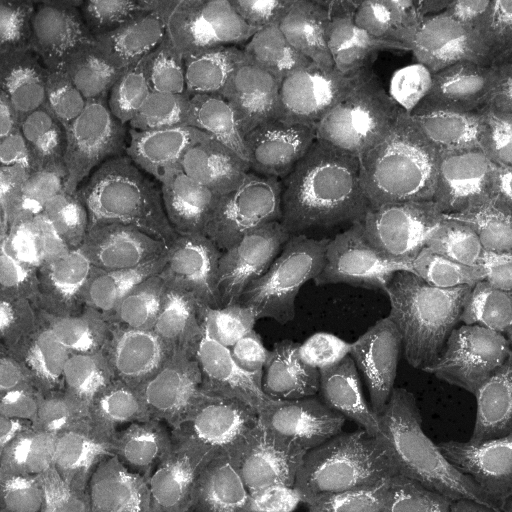
\includegraphics[width=0.92\linewidth,height=0.61\textheight,keepaspectratio]{assets/gene-examples/DNM1L-treatment-center512.png}
\end{column}
\begin{column}{0.48\textwidth}
\centering\textbf{No-guide negative control}\par\smallskip
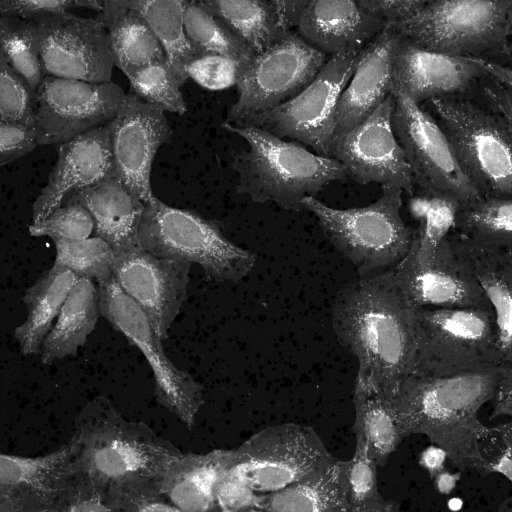
\includegraphics[width=0.92\linewidth,height=0.61\textheight,keepaspectratio]{assets/gene-examples/DNM1L-control-center512.png}
\end{column}
\end{columns}
\smallskip
{\scriptsize JUMP Mito channel; source\_13, CP-CC9-R1-02, P18 / B02, field index 0.\\
Both panels share intensity limits 187--4463. \href{https://github.com/jump-cellpainting/datasets}{JUMP data}.}
\end{frame}
% END FRAME: sec:org000000b

% BEGIN FRAME: sec:org000000f
\begin{frame}[label={sec:org000000f}]{Agents can help to get to the right data quickly}
\begin{block}{Start with a biological question}
How does disrupting mitochondrial fusion or division change cell images? Find primary studies for OPA1 and DNM1L and explain the expected phenotypes.
\end{block}
\medskip
\textbf{Build a tool to inspect the data:}\par
``Let me choose a gene KO, load its raw images beside a negative control in its plate, and zoom into cells using shared intensity limits.''
\par\bigskip
\textbf{Output:} Interactive viewer.
\end{frame}
% END FRAME: sec:org000000f

% BEGIN FRAME: demo:ai-assisted-gene-explorer
\begin{frame}[label={demo:ai-assisted-gene-explorer}]{AI-assisted tools: gene and raw-image explorer}
\begin{columns}[c,onlytextwidth]
\begin{column}{0.64\textwidth}
\centering
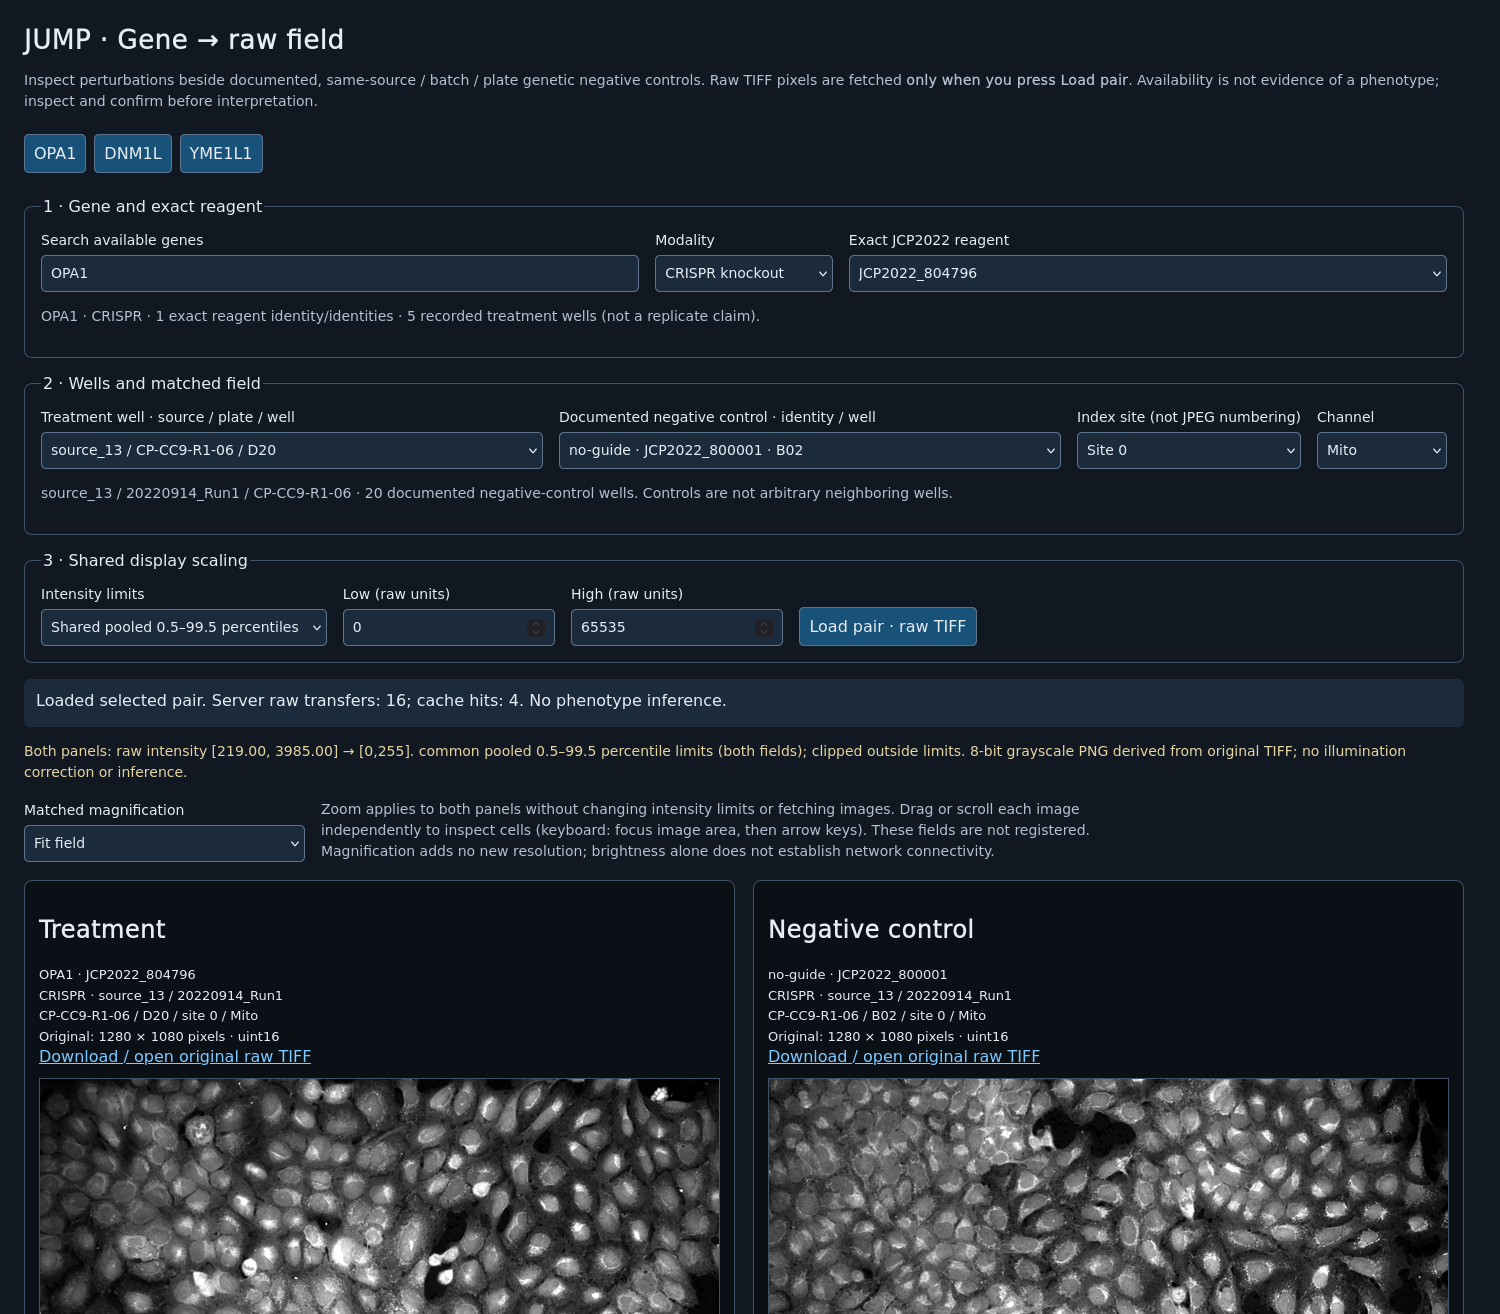
\includegraphics[width=\linewidth,height=0.78\textheight,keepaspectratio]{assets/vibe-coded/gene-explorer.png}
\end{column}
\begin{column}{0.32\textwidth}
\textbf{From a gene to its images}
\begin{itemize}
\item Select a gene and perturbation.
\item Load raw images with plate-matched controls.
\item Zoom into cells with shared intensity limits.
\item Record which differences are visible.
\end{itemize}
\end{column}
\end{columns}
\par\smallskip{\fontsize{5.5}{6.5}\selectfont Explorer images: JUMP.}
\end{frame}
% END FRAME: demo:ai-assisted-gene-explorer

% BEGIN FRAME: analysis:gene-validation
\begin{frame}[label={analysis:gene-validation}]{Validate known biology to discover new phenotypes}
\centering
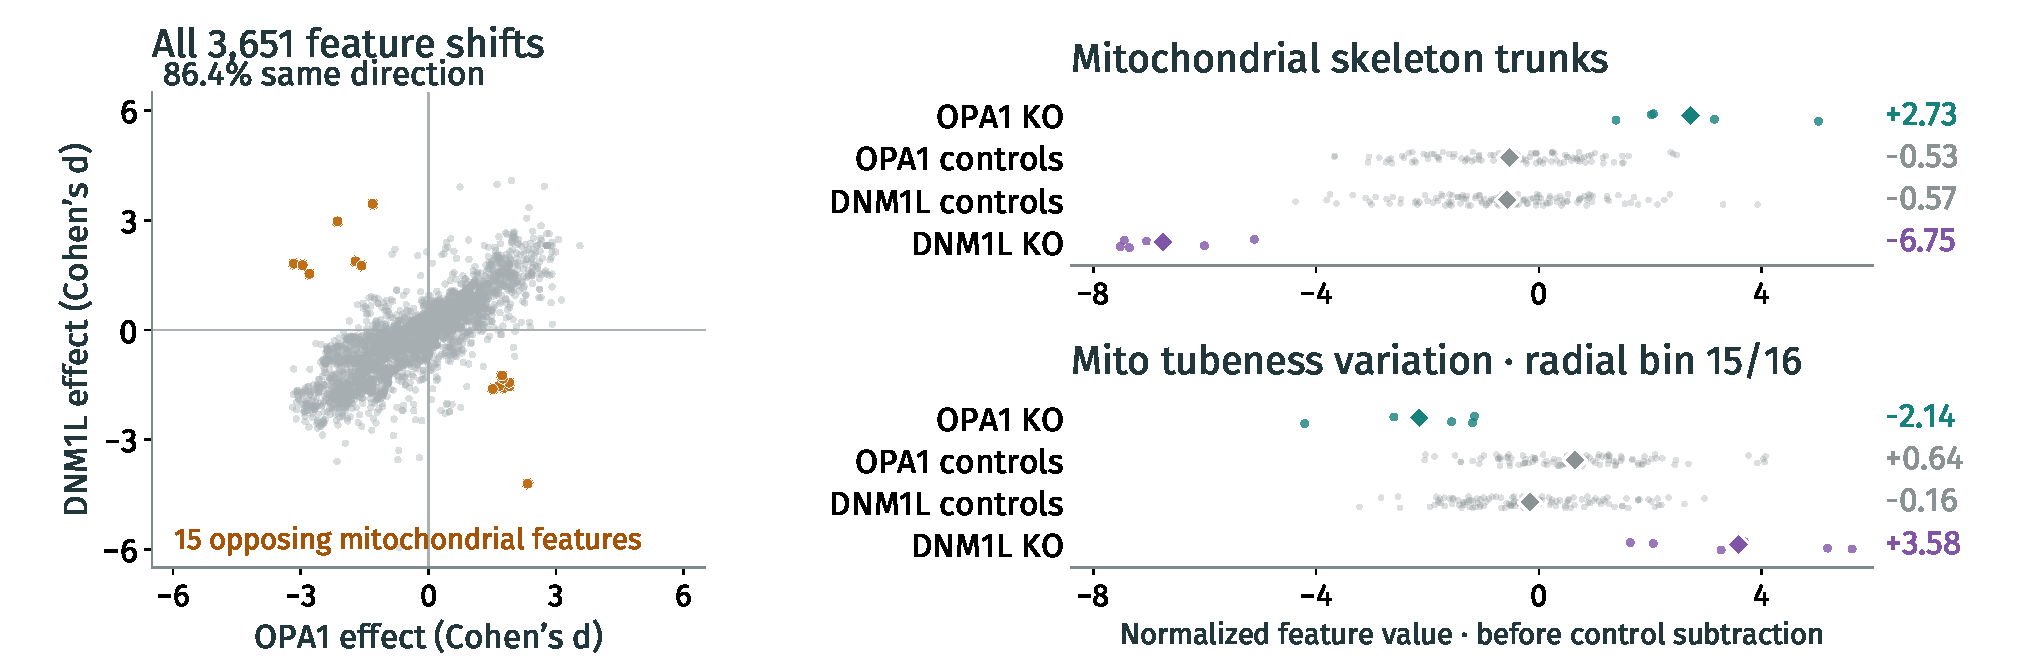
\includegraphics[width=\linewidth,height=0.66\textheight,keepaspectratio]{assets/opa1-dnm1l-analysis/feature-validation.pdf}
\par\smallskip
{\small\textbf{Shared overall shifts; opposite mitochondrial changes around the controls.}\par}
\par\smallskip
{\scriptsize\raggedright Dots: individual wells. Diamonds: group means.\par}
\end{frame}
% END FRAME: analysis:gene-validation

\section*{Applications and resources}
% BEGIN FRAME: sec:org0000012
\begin{frame}[label={sec:org0000012}]{Not just JUMP: Extract morphological profiles from your own images}
\begin{columns} [c,onlytextwidth]
\begin{column}{0.44\textwidth}
\centering
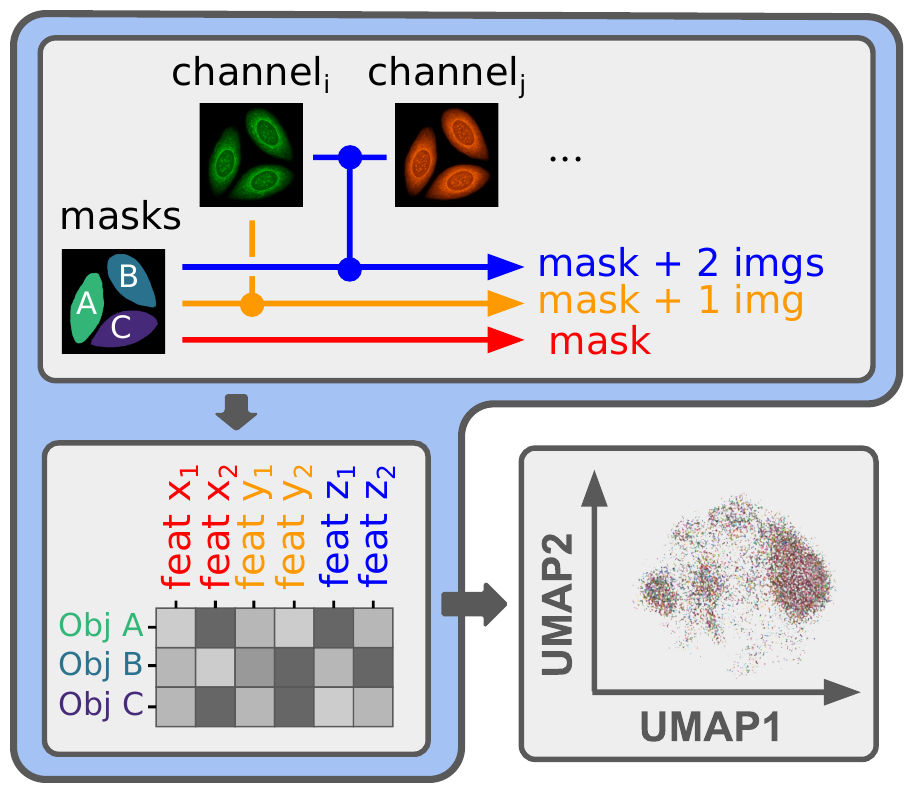
\includegraphics[width=0.98\linewidth,height=0.66\textheight,keepaspectratio]{assets/cp-measure-paper.png}
\end{column}
\begin{column}{0.53\textwidth}
\textbf{cp\_measure: feature extraction in Python}
\begin{itemize}
\item Thousands of features across channels and compartments.
\item Fits your Python pipeline.
\item Fast software to obtain interpretable morphological features ($\sim$5x CellProfiler).
\end{itemize}
\end{column}
\end{columns}

\par\smallskip\hfill{\fontsize{5.5}{6.5}\selectfont\color{gray}\href{https://arxiv.org/abs/2507.01163v1}{Adapted from Muñoz et al. (2025), Fig. 1}}
\end{frame}
% END FRAME: sec:org0000012

% BEGIN FRAME: sec:org000000e
\begin{frame}[label={sec:org000000e}]{Modern tools make image analysis more accessible}
\begin{tabular}{@{}>{\raggedright\arraybackslash}p{0.49\textwidth}>{\raggedright\arraybackslash}p{0.46\textwidth}@{}}
\textbf{Find cells, nuclei and spots} & {\small Cellpose (cells and nuclei); Spotiflow (spots)} \\[0.9em]
\textbf{Follow cells and organelles over time} & {\small Trackastra / Ultrack} \\[0.9em]
\textbf{Measure cell and organelle appearance} & {\small cp\_measure} \\[0.9em]
\textbf{Explore your results} & {\small marimo / custom app} \\[0.9em]
\end{tabular}
\end{frame}
% END FRAME: sec:org000000e

% BEGIN FRAME: sec:org0000013
\begin{frame}[label={sec:org0000013}]{Applications of JUMP and our tools across biological questions}
\begin{columns}[T,onlytextwidth]
\begin{column}{0.48\textwidth}
\begin{block}{Evaluate new lysosomal fluorescence probes}
\small Kenneth Li, University of Edinburgh\par
\begin{itemize}
\item Lysosomal acidification probes in cardiomyocytes.
\item Uptake, localization and morphology over time.
\end{itemize}
\end{block}
\end{column}
\begin{column}{0.48\textwidth}
\begin{block}{MisLocus: protein mislocalisation}
\small Johan Fredin, Carpenter-Shen Lab, Purdue University\par
\begin{itemize}
\item Which rare genetic mutations change protein location?
\item Compare microscopy of reference and variant proteins.
\end{itemize}
\end{block}
\end{column}
\end{columns}
\begin{columns}[T,onlytextwidth]
\begin{column}{0.48\textwidth}
\begin{block}{Compare imaging modalities}
\small Minh Doan, GSK Bioimaging Analytics\par
\begin{itemize}
\item Bright-field time series, Cell Painting, cell cycle and viability.
\item Which dyes and imaging methods best distinguish different mechanisms of action?
\end{itemize}
\end{block}
\end{column}
\begin{column}{0.48\textwidth}
\begin{block}{Integrated in spatial omics software}
\small Tim Treis, Theis Lab, Helmholtz-Munich\par
\begin{itemize}
\item Integration of morphological features with Squidpy.
\end{itemize}
\end{block}
\end{column}
\end{columns}
\end{frame}
% END FRAME: sec:org0000013

% \begin{frame}[label={sec:org0000014}]{MisLocus: a single-cell image benchmark}
% \small MisLocus contains $\sim$3 million cells spanning 1,541 reference/variant alleles across 282 genes, excluding controls.\par\medskip
% \begin{columns}[T,onlytextwidth]
% \begin{column}{0.54\textwidth}
% \centering
% \small Does a variant change where the protein is located?\par\medskip
% \begin{minipage}[t]{0.47\linewidth}
% \centering
% LZTR1 reference\par\smallskip
% 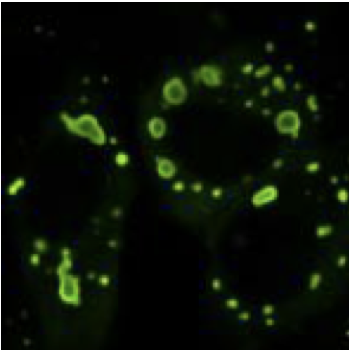
\includegraphics[width=\linewidth,keepaspectratio]{assets/mislocus-lztr1-reference.png}
% \end{minipage}\hfill
% \begin{minipage}[t]{0.47\linewidth}
% \centering
% LZTR1 G248R\par\smallskip
% 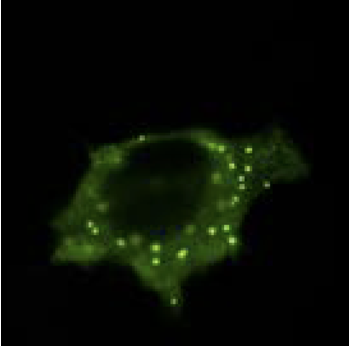
\includegraphics[width=\linewidth,keepaspectratio]{assets/mislocus-lztr1-g248r.png}
% \end{minipage}
% \end{column}
% \begin{column}{0.42\textwidth}
% \begin{block}{Protein mislocalisation}
% \begin{itemize}
% \item Compare reference and variant proteins.
% \item Test for localisation changes.
% \item Evaluate image representations.
% \end{itemize}
% \end{block}
% \end{column}
% \end{columns}\medskip
% \centering\small

% \par\smallskip\hfill{\fontsize{5.5}{6.5}\selectfont\color{gray}Images from Taipale lab}
% \end{frame}
% BEGIN FRAME: sec:org0000015
\begin{frame}[label={sec:org0000015}]{Take-home messages}
\begin{itemize}
\item Known biology helps us identify informative features and develop methods for discovery.
\item JUMP provides public Cell Painting data for around 136,000 chemical and genetic perturbations.
\item Biologists can use JUMP Hub to find tested genes and compounds, compare phenotypes and inspect images.
\item Open-source image-analysis tools extend morphological profiling to your own experiments.
\item Guides and notebooks help scientists or AI agents build analysis workflows.
\end{itemize}
\end{frame}
% END FRAME: sec:org0000015
% BEGIN FRAME: sec:org0000016
\begin{frame}[label={sec:org0000016}]{Thank you}
\centering
\begin{columns}[c,onlytextwidth]
\begin{column}{0.65\textwidth}
\centering

\includegraphics[width=0.30\linewidth,height=0.08\textheight,keepaspectratio]{assets/broad-logo.png}
\end{column}
\begin{column}{0.34\textwidth}
\centering

\includegraphics[width=0.70\linewidth,height=0.08\textheight,keepaspectratio]{assets/purdue-logo.png}
\end{column}
\end{columns}\par\smallskip
\begin{columns}[T,onlytextwidth]
\begin{column}{0.34\textwidth}
\centering\small
\textbf{Carpenter-Singh Lab}\par
Anne E. Carpenter\par
Shantanu Singh
\end{column}
\begin{column}{0.30\textwidth}
\centering\small
\textbf{Cimini Lab}\par
Beth Cimini\par
Paula Llanos
\end{column}
\begin{column}{0.34\textwidth}
\centering\small
\textbf{Carpenter-Shen Lab}\par
Anne E. Carpenter\par
Runxi Shen
\end{column}
\end{columns}\par\smallskip

\includegraphics[width=0.98\linewidth,height=0.50\textheight,keepaspectratio]{assets/jump-partners.png}\par\medskip
{\small Work on cp\_measure and JUMP-lite was supported by GSK and NIH MIRA (R35 GM122547).}\par
\end{frame}
% END FRAME: sec:org0000016

% BEGIN FRAME: sec:org0000018
\begin{frame}[label={sec:org0000018}]{JUMP Hub and slides}
\begin{columns}[T,onlytextwidth]
\begin{column}{0.48\textwidth}
\centering
\href{https://broadinstitute.github.io/jump_hub/}{JUMP Hub}\par\smallskip
\href{https://broadinstitute.github.io/jump_hub/}{
\includegraphics[width=40mm]{assets/qr-jump-hub.png}}\par\smallskip
\href{https://broad.io/jump}{\texttt{broad.io/jump}}
\end{column}
\begin{column}{0.48\textwidth}
\centering
\href{https://raw.githubusercontent.com/afermg/2026_11_10_jump_hub/main/slides.pdf}{Slides (PDF)}\par\smallskip
\href{https://raw.githubusercontent.com/afermg/2026_11_10_jump_hub/main/slides.pdf}{
\includegraphics[width=40mm]{assets/qr-slides.png}}
\end{column}
\end{columns}
\end{frame}
% END FRAME: sec:org0000018

\section*{Additional slides}
\label{sec:org000001d}

% BEGIN FRAME: sec:org0000017
\begin{frame}[label={sec:org0000017}]{References}
{\footnotesize All named tools and models below are clickable.}
\medskip
\begin{columns}[T,onlytextwidth]
\begin{column}{0.32\textwidth}
\footnotesize
\textbf{Assay, data and resources}
\begin{itemize}
\item \href{https://doi.org/10.1038/nprot.2016.105}{Cell Painting (Bray, 2016)}; \href{https://doi.org/10.1038/s41573-020-00117-w}{profiling review (2021)}.
\item \href{https://jump-cellpainting.broadinstitute.org/}{JUMP consortium}; \href{https://github.com/jump-cellpainting/datasets/tree/016e865fa0691244e0860943e41c7d6a88ed2580/metadata}{counts}; \href{https://github.com/broadinstitute/jump_hub/blob/e742f5aa37472eb17f326ba8315d22b27e58f330/explanations/data_description.md}{centers}; \href{https://github.com/jump-cellpainting/datasets/blob/016e865fa0691244e0860943e41c7d6a88ed2580/stats/cpg0016_source_images_tiff_count.csv}{images}.
\item \href{https://arxiv.org/abs/2608.07632v3}{JUMP-lite paper}; \href{https://github.com/afermg/JUMP_lite}{data/code}.
\item \href{https://broadinstitute.github.io/jump_hub/}{JUMP Hub}; \href{https://broadinstitute.github.io/jump_hub/howto/interactive/1_jumprr_steps.html}{how-to guides}; \href{https://broadinstitute.github.io/jump_hub/howto/notebooks/0_overview.html}{notebooks}.
\item \href{https://ciminilab.github.io/GuideToCellPainting/}{Guide to Cell Painting}.
\end{itemize}
\end{column}
\begin{column}{0.32\textwidth}
\footnotesize
\textbf{Image-analysis toolbox}
\begin{itemize}
\item \href{https://github.com/afermg/cp_measure}{cp\_measure}; \href{https://arxiv.org/abs/2507.01163v1}{paper}.
\item \href{https://cellprofiler.org/}{CellProfiler}; \href{https://doi.org/10.1186/gb-2006-7-10-r100}{paper}.
\item \href{https://github.com/MouseLand/cellpose}{Cellpose}; \href{https://github.com/stardist/stardist}{StarDist}.
\item \href{https://github.com/weigertlab/spotiflow}{Spotiflow}: spot detection.
\item \href{https://github.com/weigertlab/trackastra}{Trackastra}; \href{https://github.com/royerlab/ultrack}{Ultrack}.
\item \href{https://marimo.io/}{marimo}; \href{https://docs.astral.sh/uv/}{uv}.
\item \href{https://squidpy.readthedocs.io/}{Squidpy}; \href{https://github.com/cmap/morpheus.js}{Morpheus}.
\end{itemize}
\end{column}
\end{columns}
\end{frame}
% END FRAME: sec:org0000017

% BEGIN FRAME: sec:org0000003
\begin{frame}[label={sec:org0000003}]{Morphological profiling: How to turn images into profiles}
Start with a simple question: are control and perturbed cells different?

\begin{columns}[T,onlytextwidth]
\begin{column}{0.48\textwidth}
\begin{block}{Classical features (e.g., CellProfiler)}
\begin{itemize}
\item Size, shape, intensity, texture and relationships between channels and objects.
\item Interpretable but partially redundant.
\end{itemize}
\end{block}
\end{column}
\begin{column}{0.48\textwidth}
\begin{block}{Learned representations}
\begin{itemize}
\item Features learned from images by neural networks (deep learning).
\item Non-redundant numerical vectors (embeddings).
\end{itemize}
\end{block}
\end{column}
\end{columns}
\end{frame}
% END FRAME: sec:org0000003

% BEGIN FRAME: sec:org0000004
\begin{frame}[label={sec:org0000004}]{Words as vectors: word2vec}
\par
{\centering\small Learning can be viewed as compression\par}
\smallskip

\begin{center}
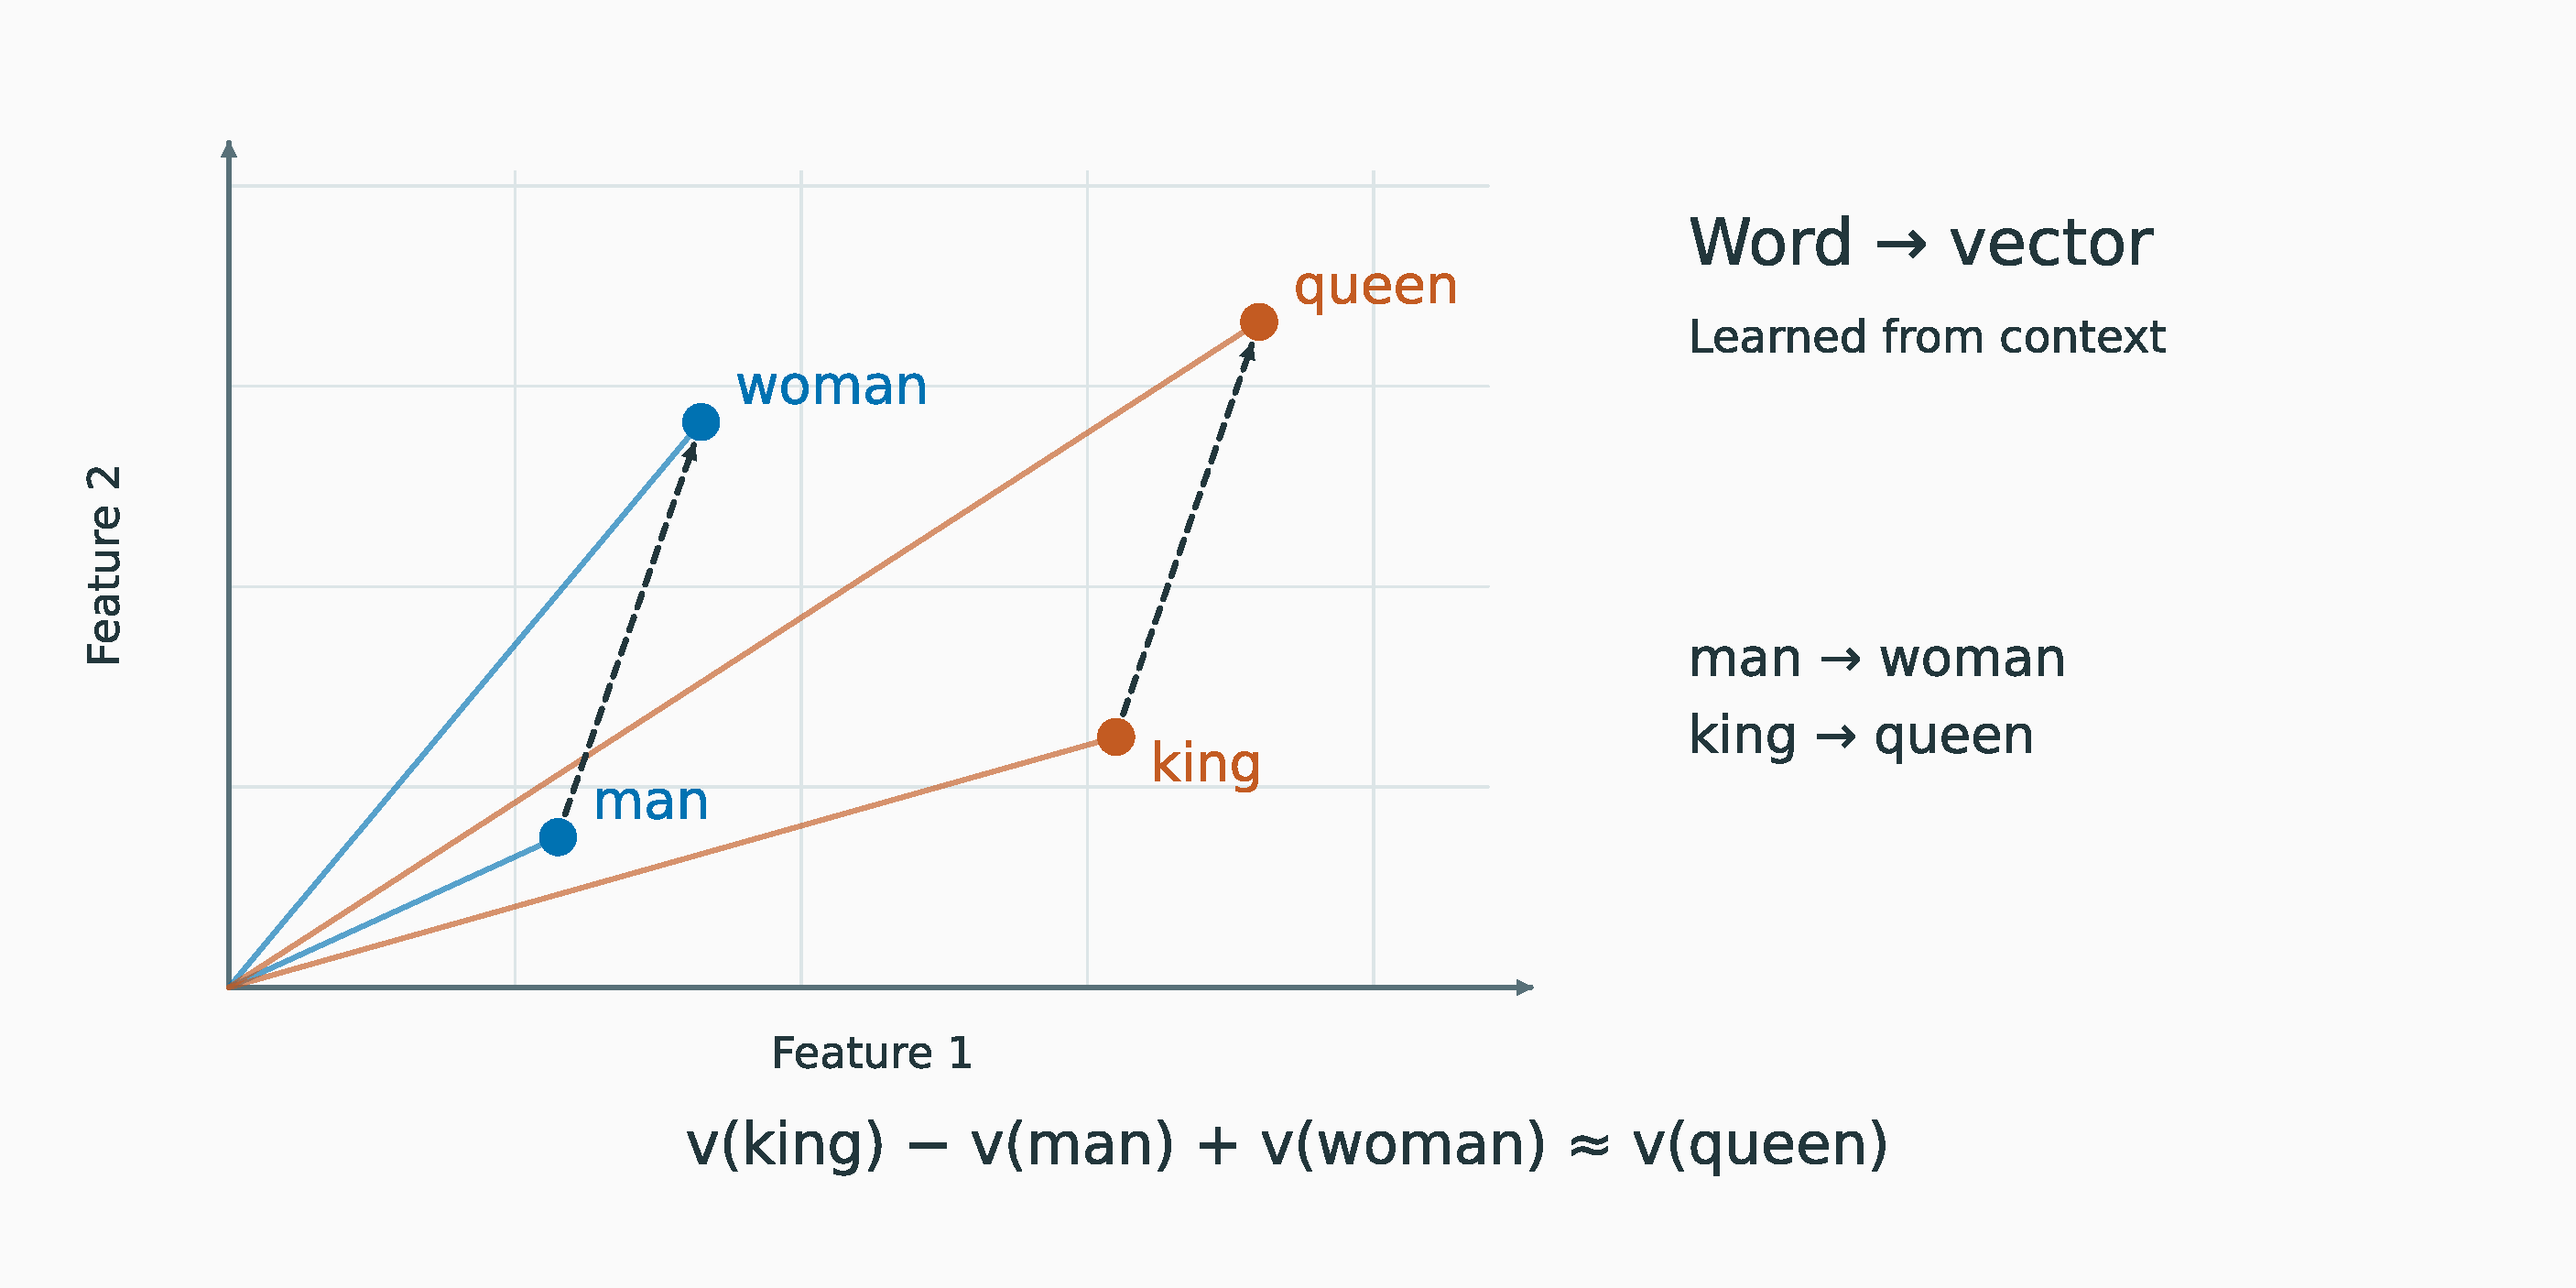
\includegraphics[keepaspectratio,width=0.99\linewidth,height=0.70\textheight]{assets/word2vec-king-queen.pdf}
\end{center}

\hfill{\scriptsize\href{https://arxiv.org/abs/1301.3781}{Mikolov et al. (2013)}}
\end{frame}
% END FRAME: sec:org0000004

% BEGIN FRAME: sec:org0000005
\begin{frame}[label={sec:org0000005}]{From words to cells: vectors for comparison}
\begin{center}
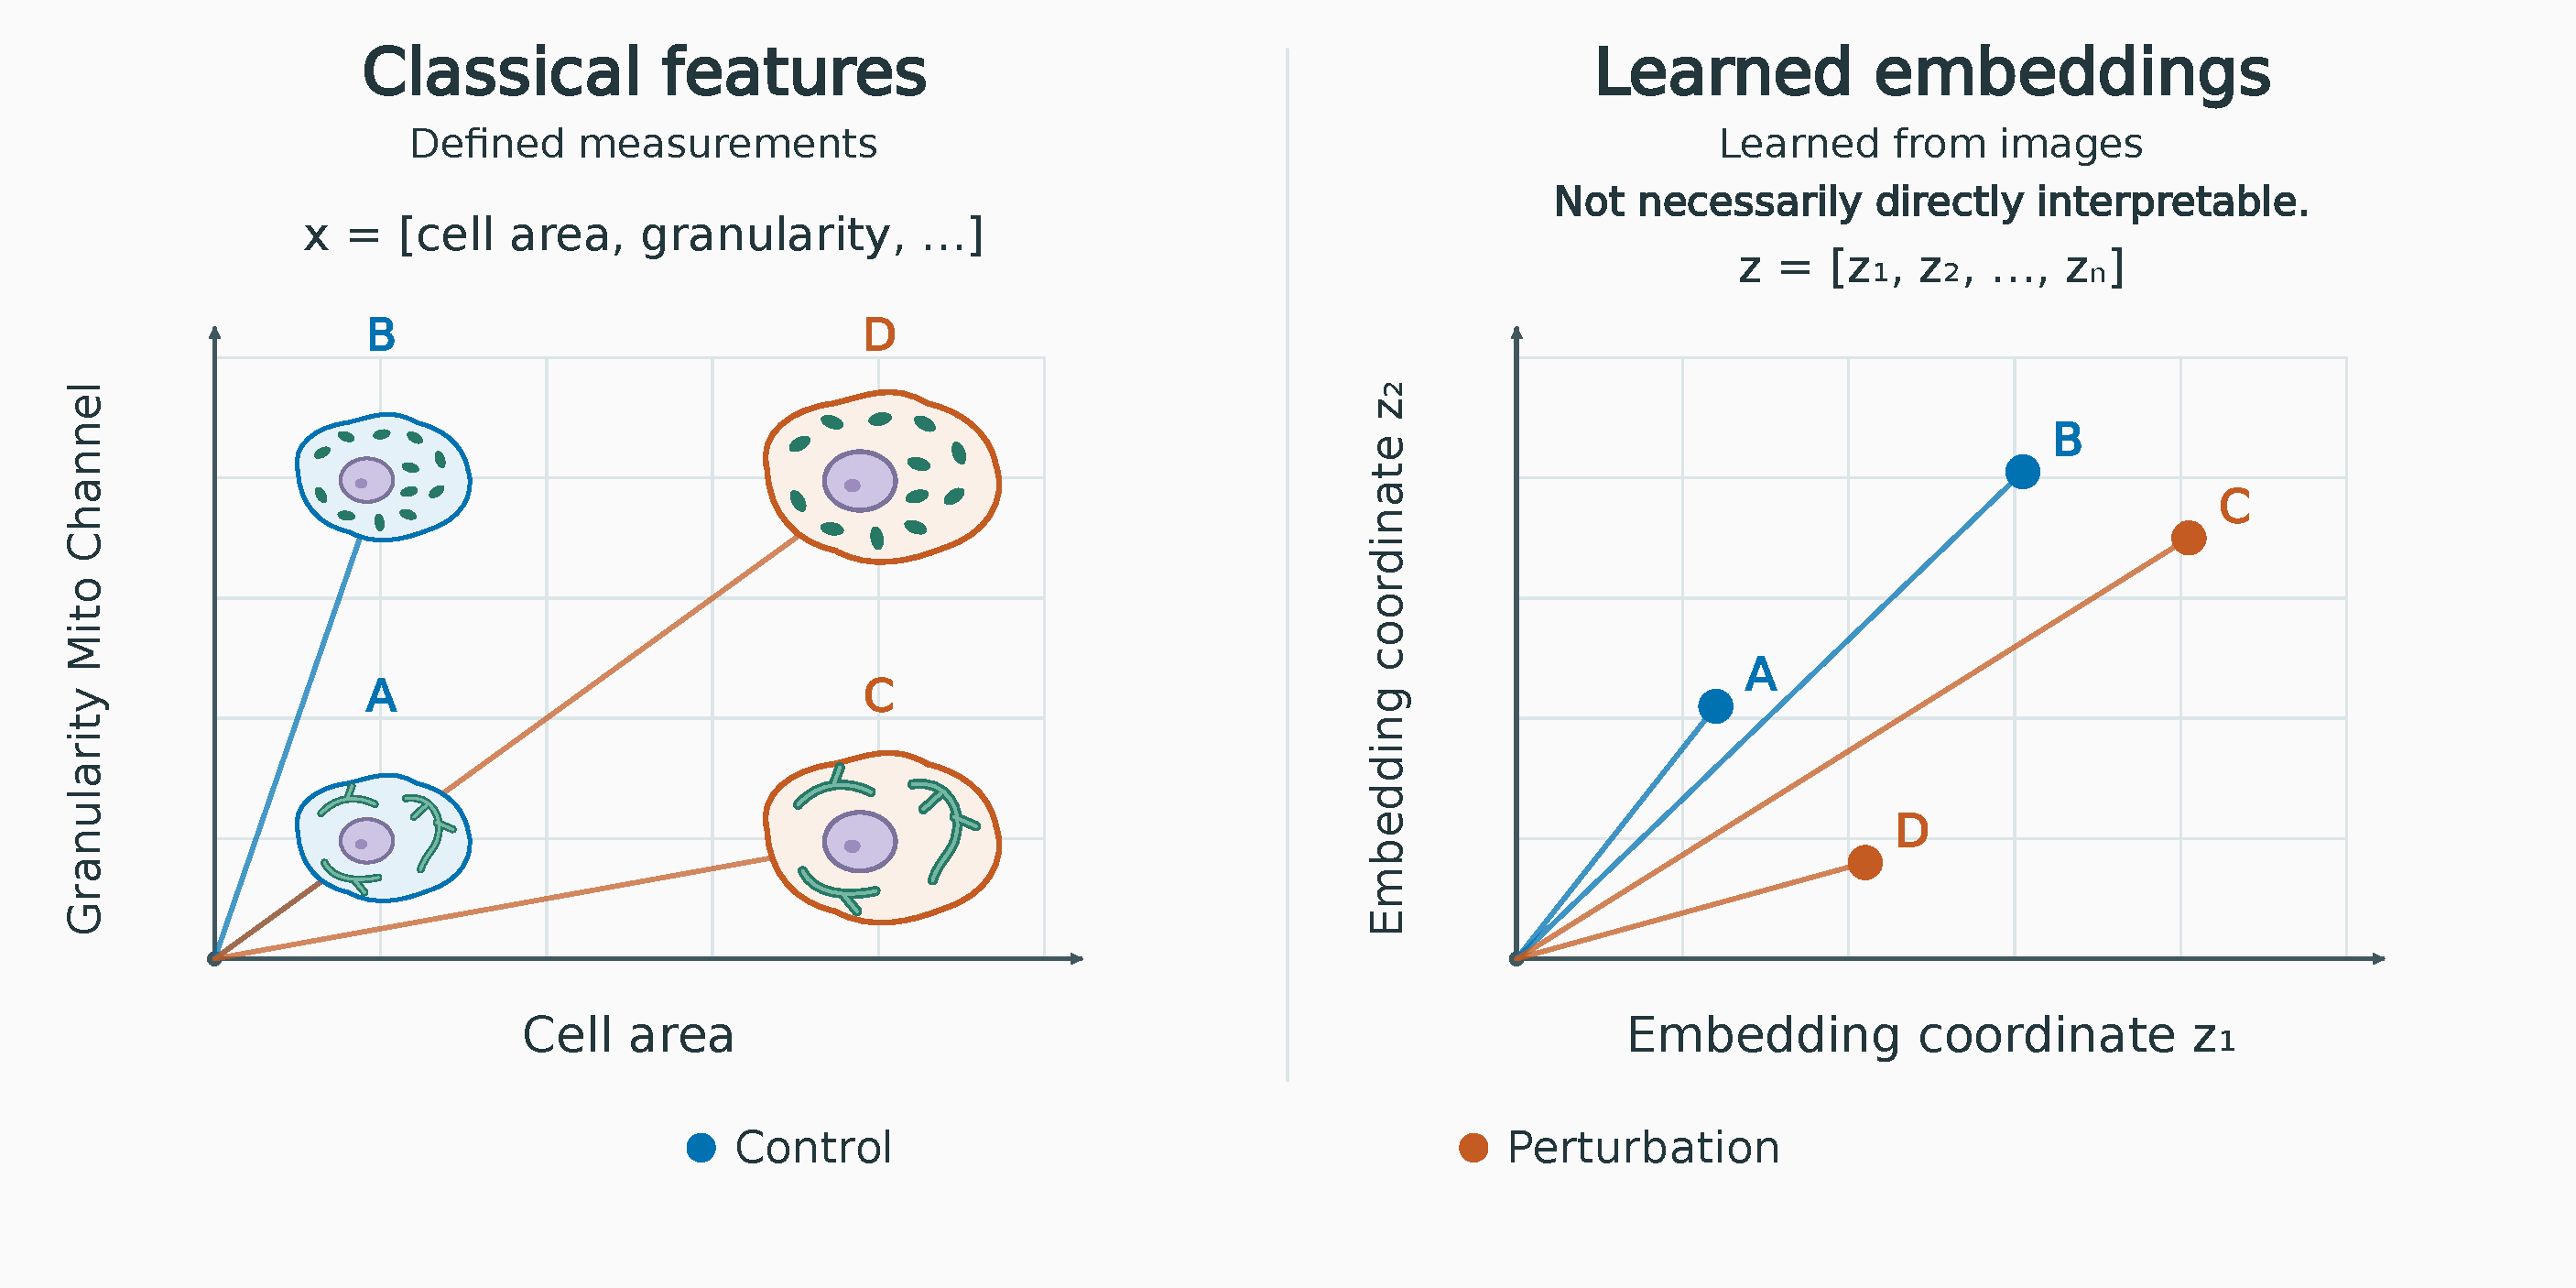
\includegraphics[keepaspectratio,width=0.99\linewidth,height=0.83\textheight]{assets/vector-control-perturbation.pdf}
\end{center}
\end{frame}
% END FRAME: sec:org0000005

% BEGIN FRAME: sec:org0000011
\begin{frame}[label={sec:org0000011}]{Positive controls contextualize perturbations in both learned and classical representations}
\begin{center}
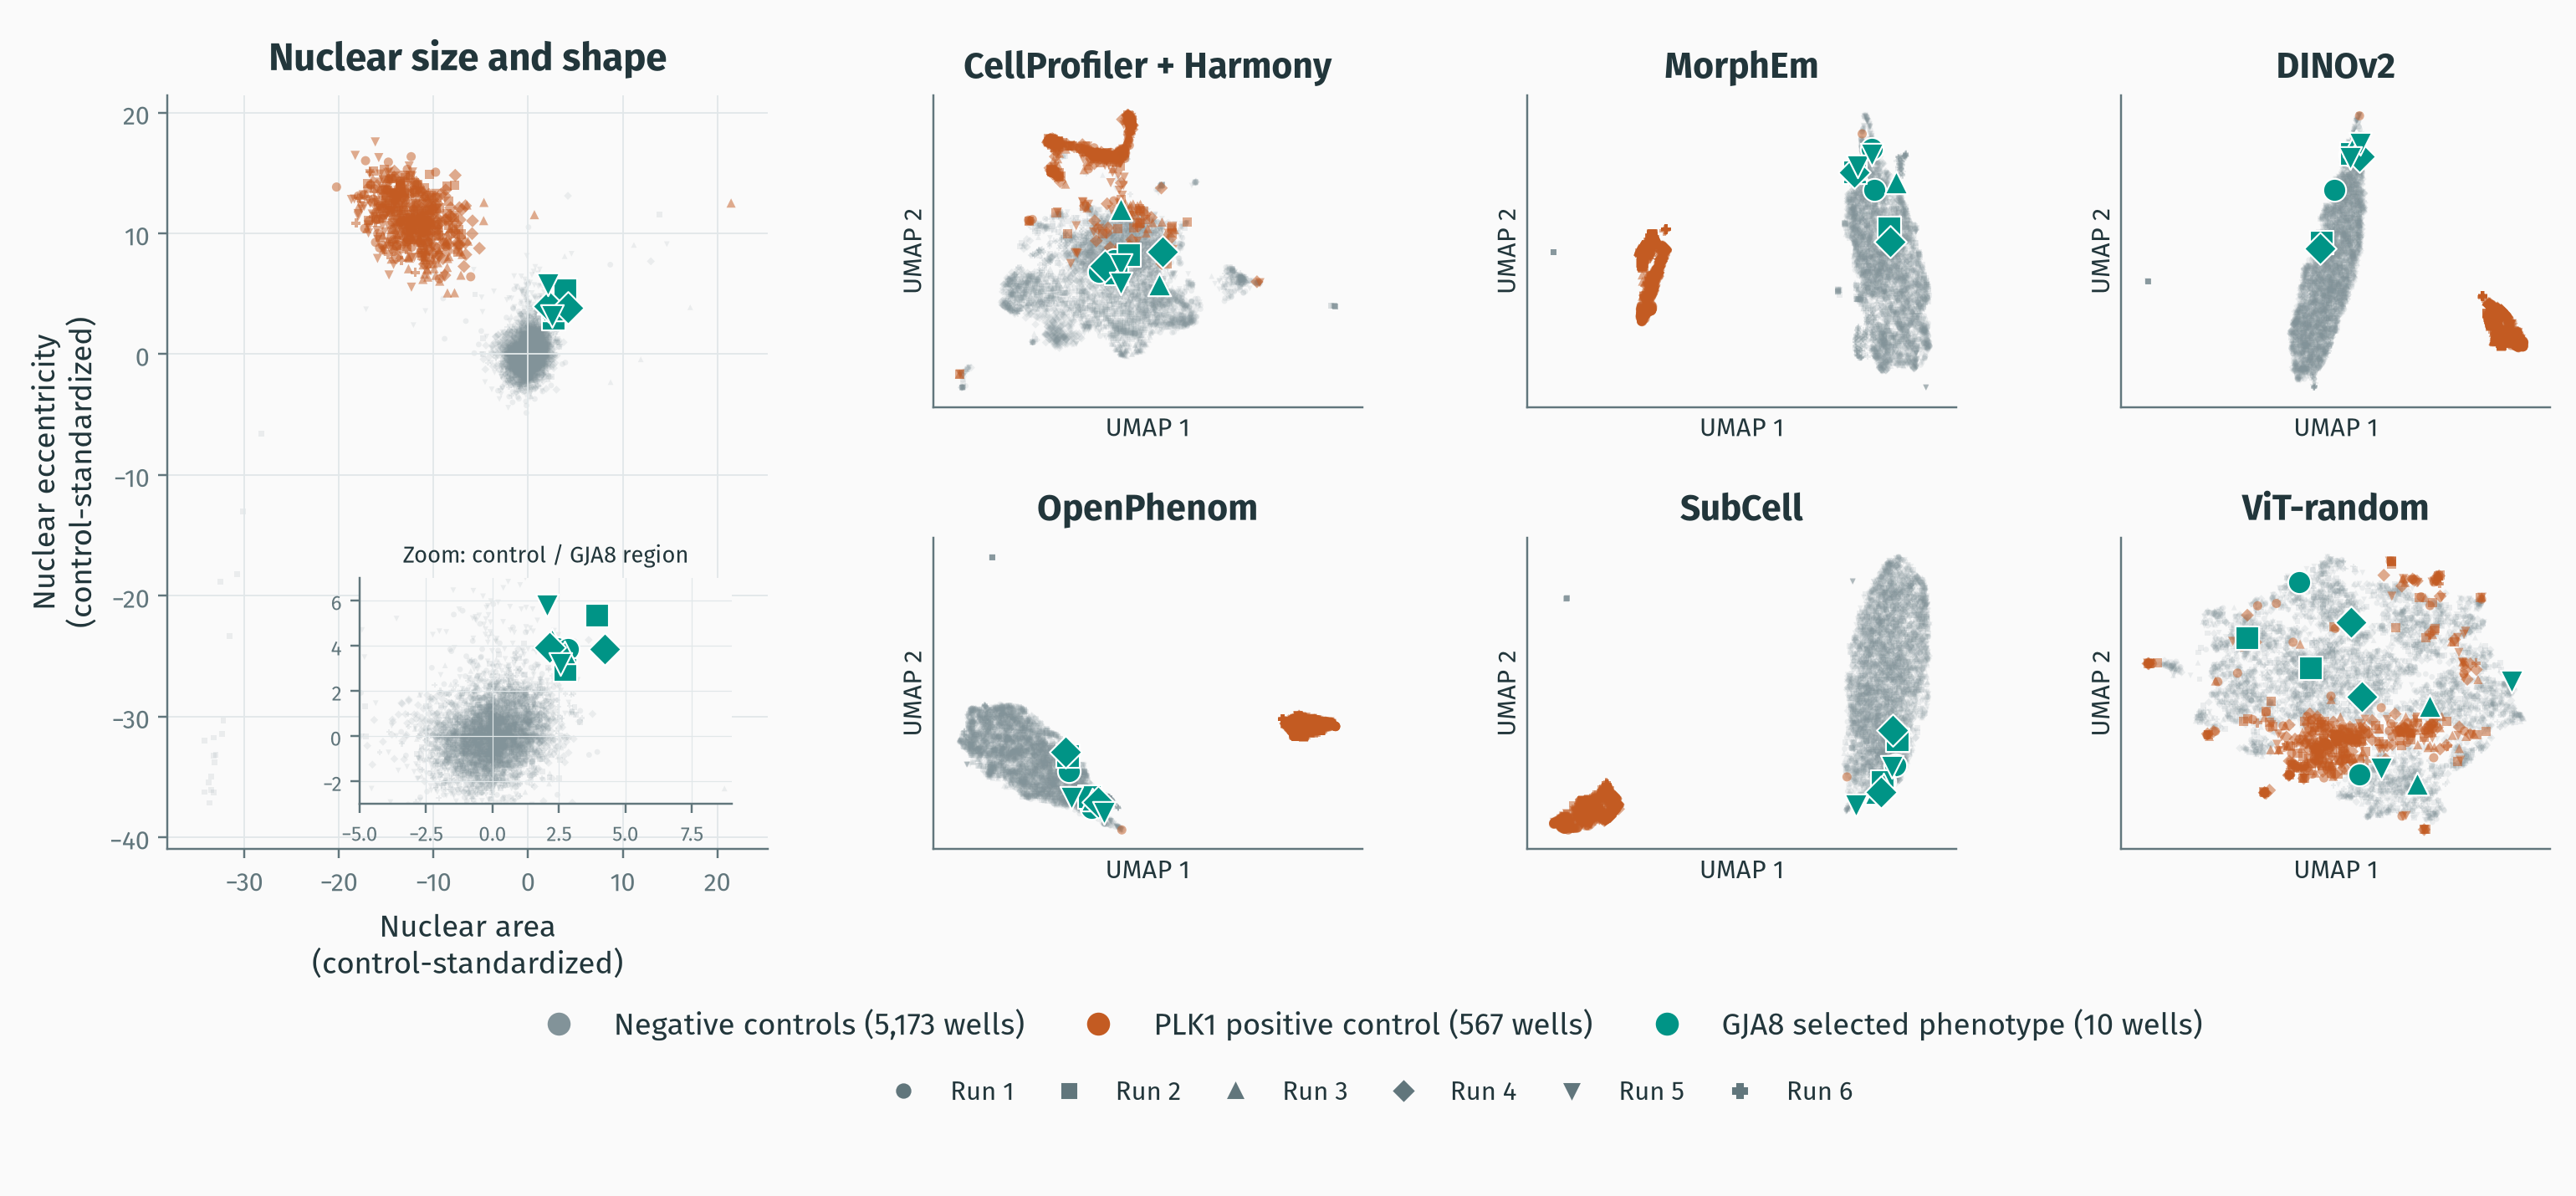
\includegraphics[keepaspectratio,width=0.94\linewidth,height=0.80\textheight]{assets/real-embeddings-combined.png}
\end{center}

\hfill{\fontsize{5.5}{6.5}\selectfont\color{gray}\href{https://arxiv.org/abs/2608.07632v3}{Data: JUMP-lite (2026)}; models: \href{https://huggingface.co/CaicedoLab/MorphEm}{MorphEm}, \href{https://github.com/facebookresearch/dinov2}{DINOv2}, \href{https://huggingface.co/recursionpharma/OpenPhenom}{OpenPhenom}, \href{https://github.com/CellProfiling/subcell-embed}{SubCell}; \href{https://github.com/broadinstitute/jump-profiling-recipe/tree/a917fa79342ff92cf0ea05d6d9174d9028a90f8f}{CellProfiler/Harmony recipe}}
\end{frame}
% END FRAME: sec:org0000011

% BEGIN FRAME: sec:org000001a
\begin{frame}[label={sec:org000001a}]{JUMP-lite: a compact benchmark}
\begin{columns}[c,onlytextwidth]
\begin{column}{0.52\textwidth}
\centering
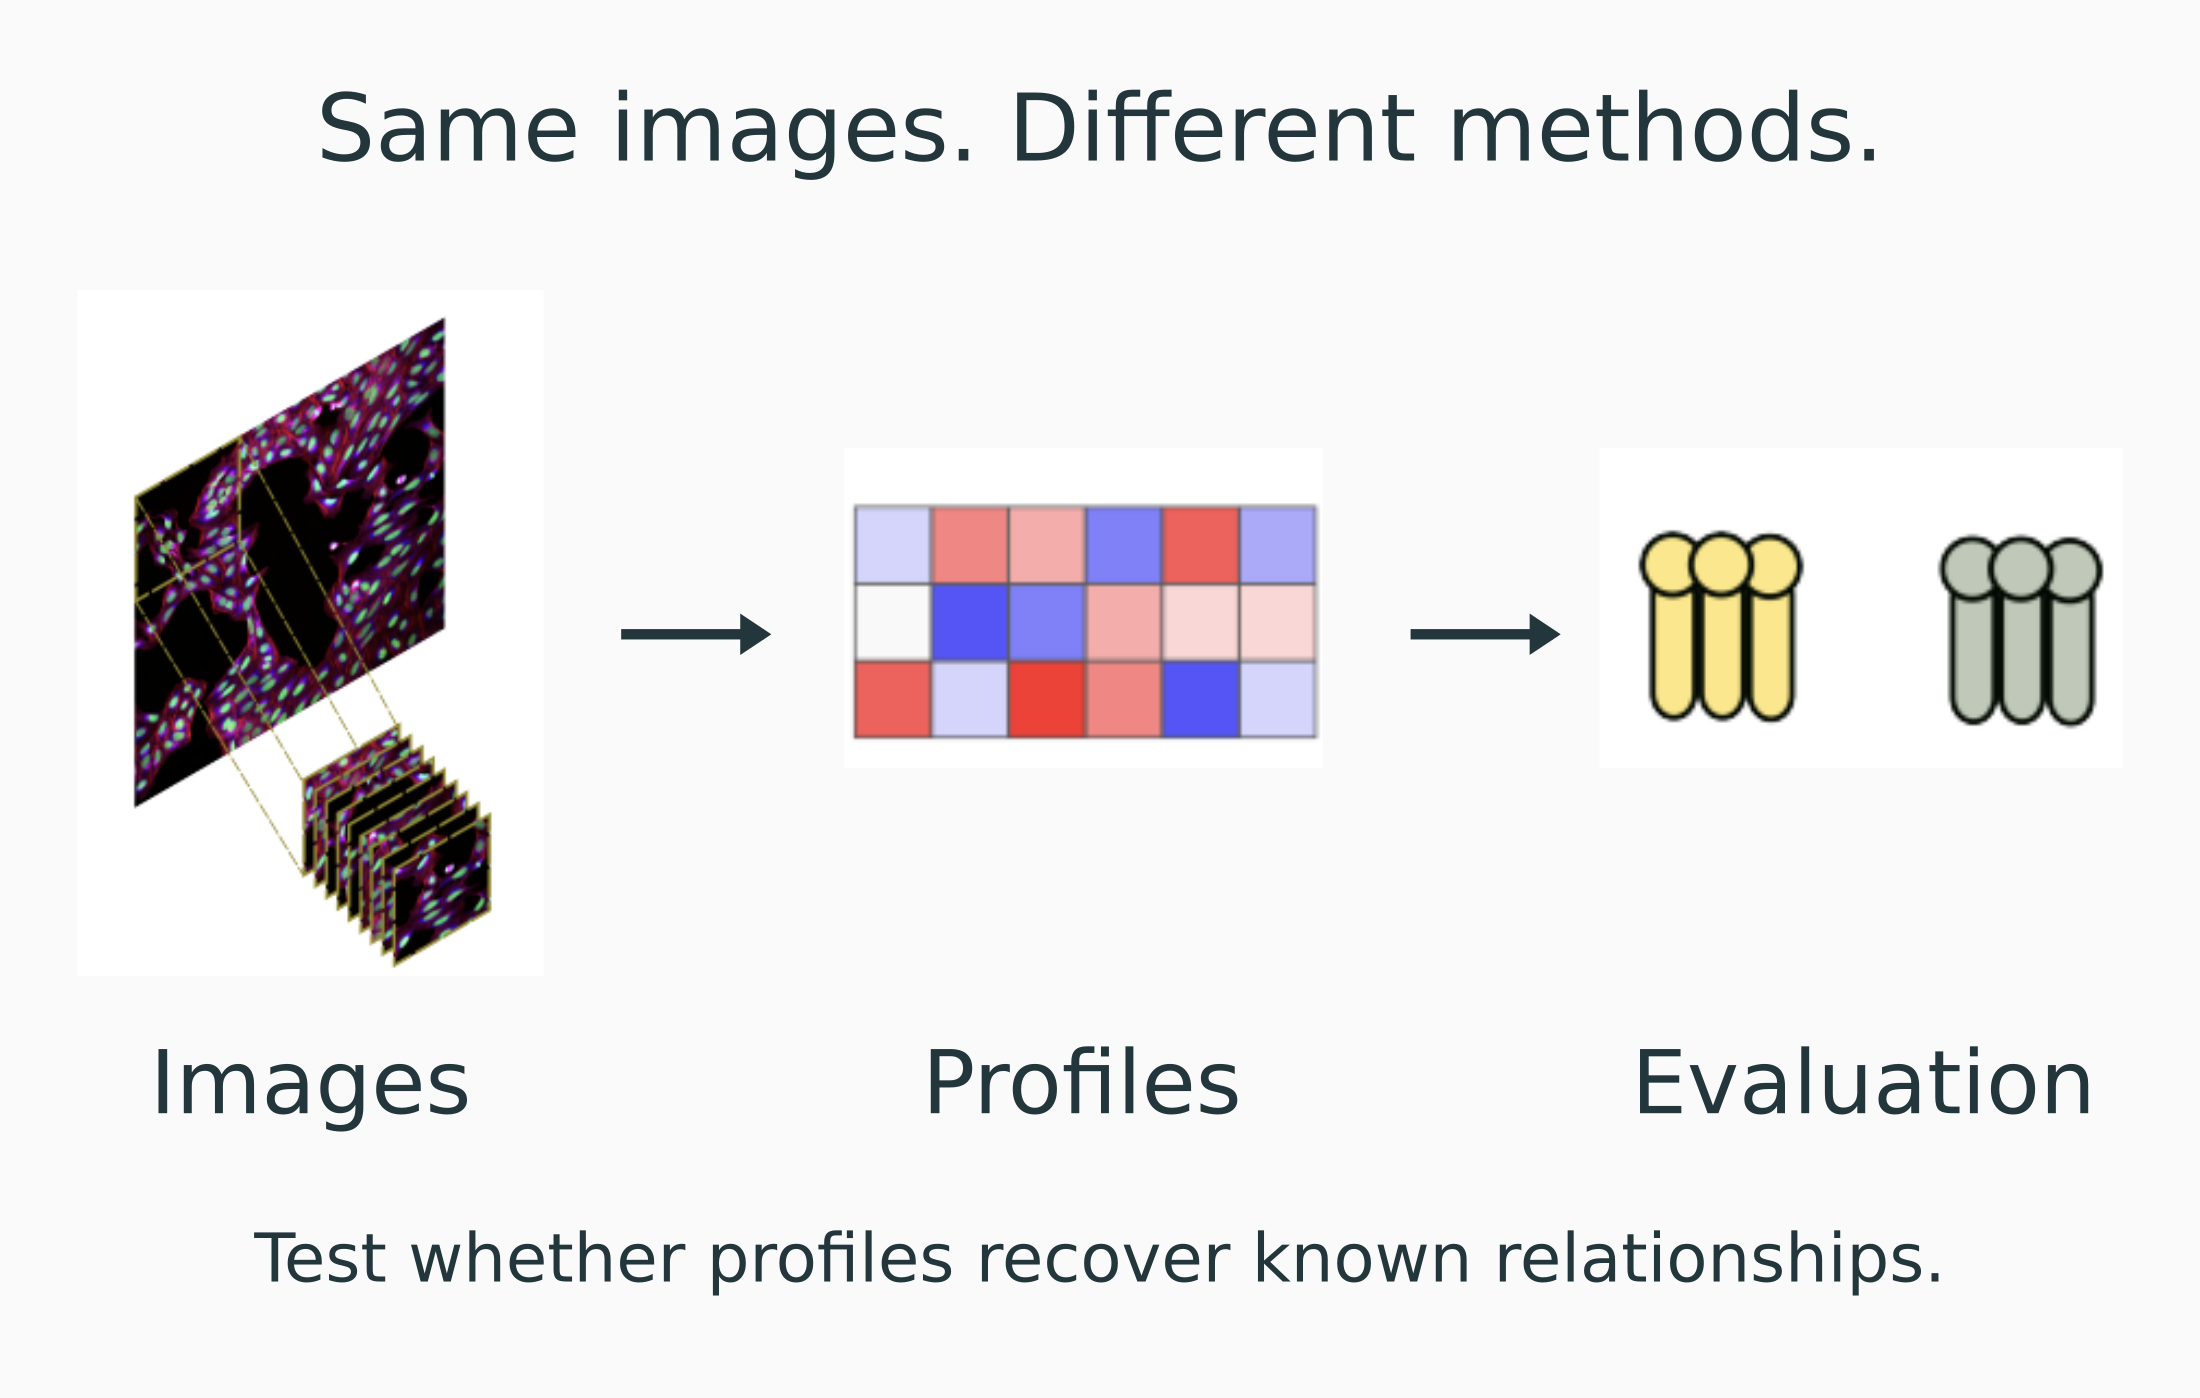
\includegraphics[width=\linewidth]{assets/jump-lite-workflow.png}
\end{column}
\begin{column}{0.46\textwidth}
\centering
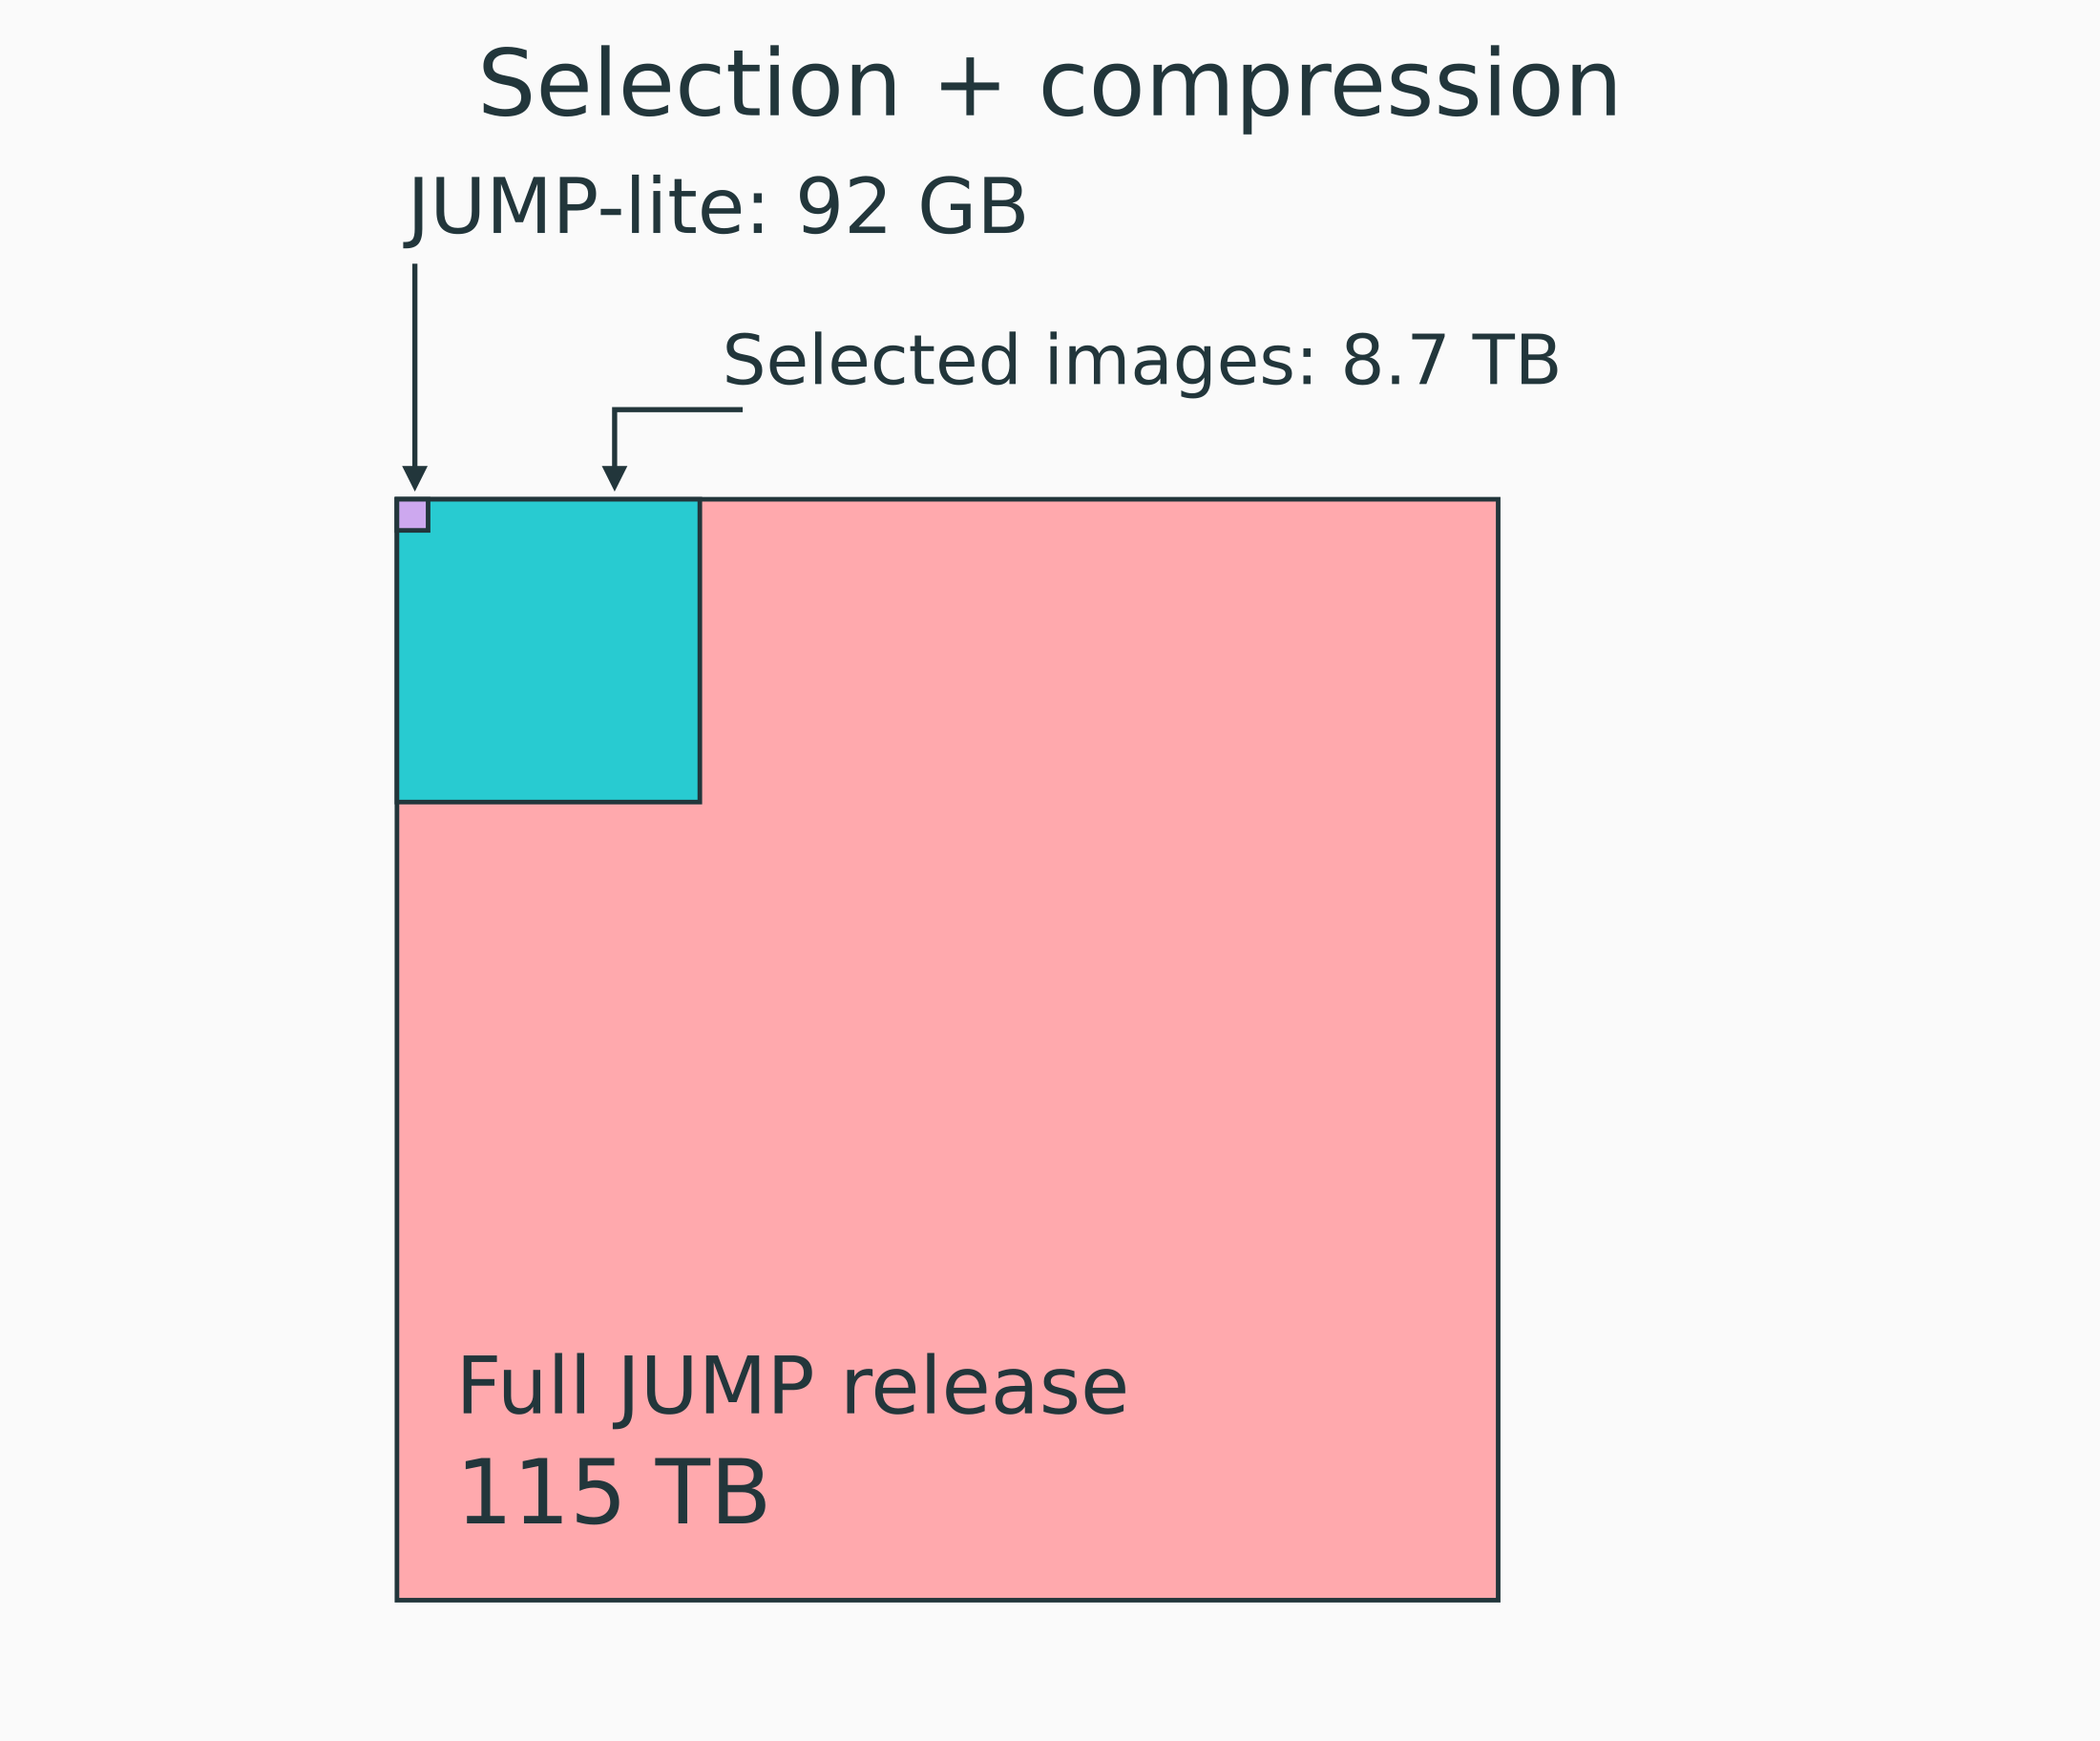
\includegraphics[width=\linewidth,height=0.76\textheight,keepaspectratio]{assets/jump-lite-squares.png}
\end{column}
\end{columns}
\medskip
\centering
{\footnotesize Same selected images: 8.7 TB $\rightarrow$ 92 GB ($\sim$94$\times$ smaller; lossy JPEG XL).}

\par\smallskip\hfill{\fontsize{5.5}{6.5}\selectfont\color{gray}\href{https://arxiv.org/abs/2608.07632v3}{Adapted from Muñoz et al. (2026)}}
\end{frame}
% END FRAME: sec:org000001a
% BEGIN FRAME: sec:org000001b
\begin{frame}[label={sec:org000001b}]{Nahual: swap models within one workflow}
\centering
{\Large\bfseries Swap models. Keep your workflow.}\par\bigskip
\renewcommand{\arraystretch}{1.8}
\begin{tabular}{@{}l l@{}}
\textbf{Image features} & \fbox{DINOv2}\ $\leftrightarrow$\ \fbox{DINOv3}\ $\leftrightarrow$\ \fbox{OpenPhenom}\ $\leftrightarrow$\ \fbox{MorphEm} \\
\textbf{Segmentation} & \fbox{Cellpose}\ $\leftrightarrow$\ \fbox{StarDist} \\
\textbf{Spot detection} & \fbox{Spotiflow} \\
\textbf{Tracking} & \fbox{Trackastra}\ $\leftrightarrow$\ \fbox{Ultrack}
\end{tabular}
\end{frame}
% END FRAME: sec:org000001b
% BEGIN FRAME: sec:org000001c
\begin{frame}[label={sec:org000001c}]{JUMP-lite: comparing image representations}
\centering\small
Recover replicate perturbations and known biological relationships.\par\smallskip
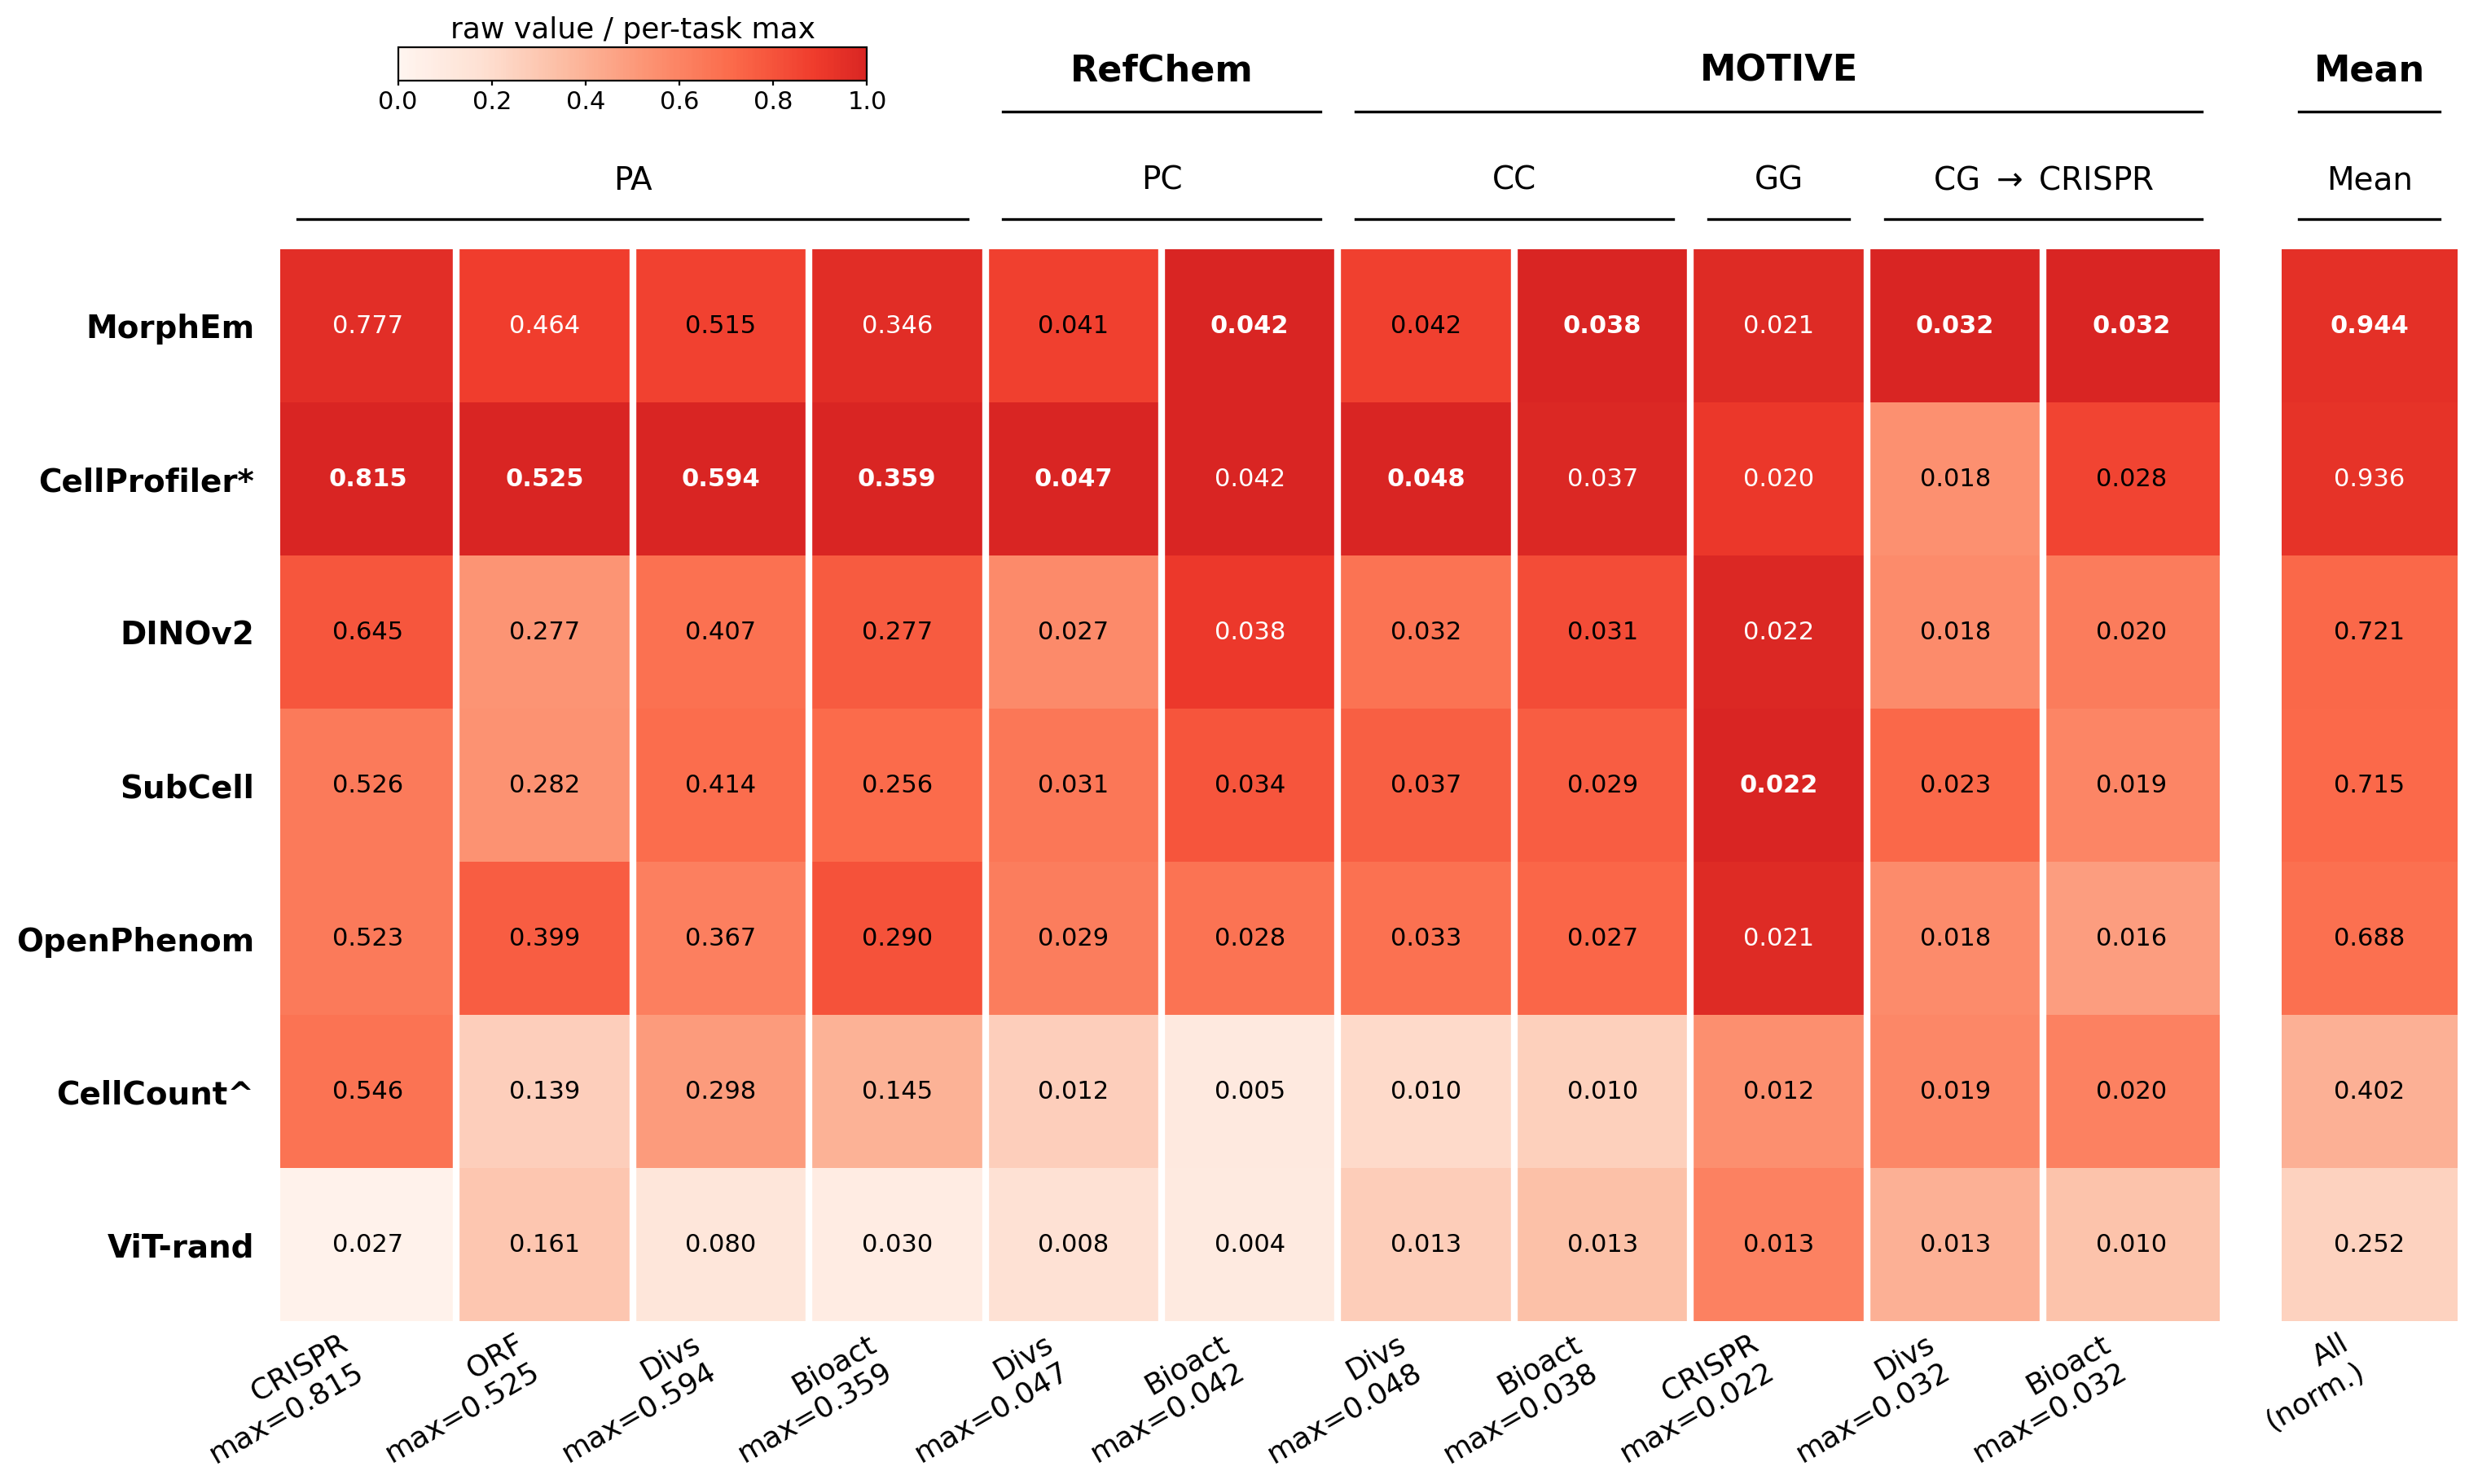
\includegraphics[width=0.99\linewidth,height=0.73\textheight,keepaspectratio]{assets/jump-lite-model-comparison.png}\par\smallskip
{\scriptsize Raw images; colors normalized within each task. CellProfiler/count references use more sites per well.\par}
{\fontsize{5.5}{6.5}\selectfont\color{gray}\hfill\href{https://arxiv.org/abs/2608.07632v3}{Adapted from Muñoz et al. (2026), Figure 5}\par}
\end{frame}
% END FRAME: sec:org000001c
% BEGIN FRAME: backup:recorded-cell-browser
\begin{frame}[label={backup:recorded-cell-browser}]{Backup: explore cell subpopulations}
Interactive marimo notebook --- separate recorded example
\begin{center}
\href{https://doi.org/10.5281/zenodo.23462248}{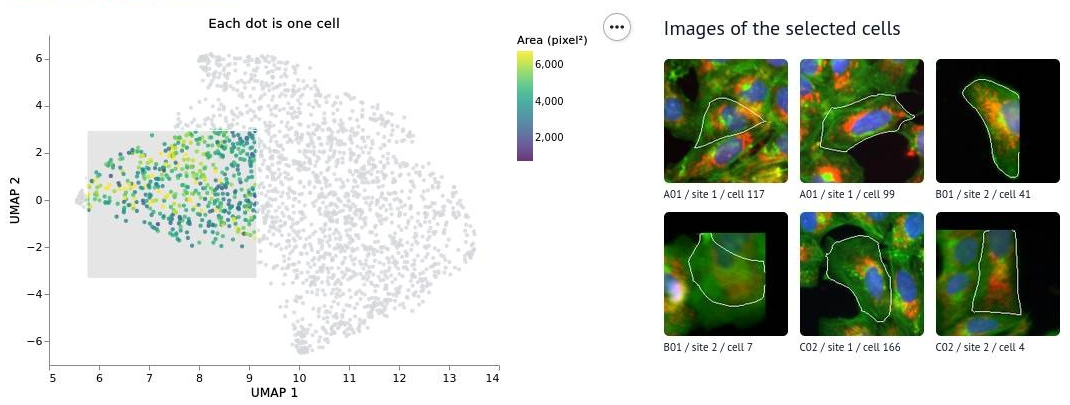
\includegraphics[width=0.85\linewidth,height=0.59\textheight,keepaspectratio]{assets/demo-selection-545.png}}
\end{center}
{\small Each dot is a cell: 2,223 from one Target-2 plate. Shown selection: 545 cells. Inspect images, area and other features.}
\par\smallskip\hfill{\fontsize{5.5}{6.5}\selectfont\color{gray}\href{https://doi.org/10.5281/zenodo.23462248}{Source: Muñoz (2026), JUMP Target-2 notebook recording}}
\end{frame}
% END FRAME: backup:recorded-cell-browser
% BEGIN FRAME: backup:recorded-second-selection
\begin{frame}[label={backup:recorded-second-selection}]{Backup: compare another cell selection}
\begin{center}
\href{https://doi.org/10.5281/zenodo.23462248}{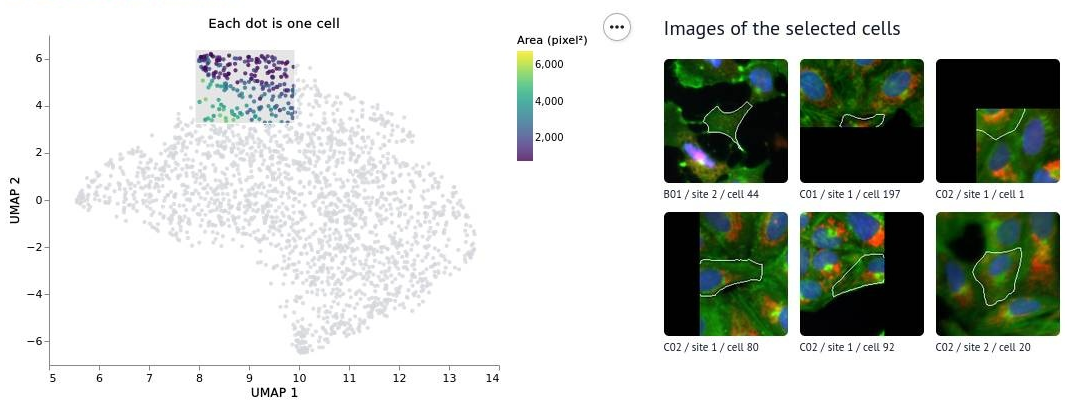
\includegraphics[width=0.96\linewidth,height=0.51\textheight,keepaspectratio]{assets/demo-selection-224.png}}
\end{center}
\begin{itemize}
\item Second selection: 224 cells; compare images and measurements.
\item Not the compound queries; no treatment/control assignments in this example.
\end{itemize}
\par\smallskip\hfill{\fontsize{5.5}{6.5}\selectfont\color{gray}\href{https://doi.org/10.5281/zenodo.23462248}{Source: Muñoz (2026), JUMP Target-2 notebook recording}}
\end{frame}
% END FRAME: backup:recorded-second-selection
\end{document}
